%%%%%%%%%%%%%%%%%%%%%%%%
%
% $Autor: Wings $
% $Datum: 2020-07-24 09:05:07Z $
% $Pfad: GDV/Vortraege/latex - Ausarbeitung/Kapitel/Einleitung.tex $
% $Version: 4732 $
%
%%%%%%%%%%%%%%%%%%%%%%%%

\chapter{Introduction}
\label{Introduction}
\section{General}

An accurate Gait Pattern analysis can at the moment only be carriered out by health professionals  and is not available to individuales, even though that a healthy gait pattern reduces the risk of having back problems or even bad injuries especially for older poeple. 
analysing the gait pattern also gives us information about the person´s previous accidents or even about current neuronal problem as changes of gait patterns could in fact be a symptom of some sicknesses like Parkinson.

the long term goal of this project would be to anable individuales analyse their own gait pattern and recognise if there is something wrong with them at a reasonable price Tag. 
but for this paper the goal would be to use IMU sensors to collect information about the gait and identify if the person is walking, running or jumping.

As  hardware an Arduino Nano BLE 33  including an IMU Sensor will be used to collect and process the data, TinyML will be used because of the limited memory of the Embedded System, TensorFlow tools to process and load data (build or train the model.) TensorFlow Lite is then used to provide the ability to perform predictions on the trained model (load the model not to train the model). 
the tool created should be placed on the thigh in a pocket, as it was shows in \cite{AbhayasingheMurray:2014} anaysing one thigh is enough to accuratly detect the movement of one leg and to predict movements of the other one. IMU sensors should detect the angle of the thigh movement and it shoud then be saved on the hardware and analysed comparing the angle´s waveform to the previous ones registred during the research.\\

the hardware used has a limited memory, using tinyML helps us avoid this problem. 
Energy source is also a challenge, since the tool is to be carried arround, it has to have a portable source of energy. Using a battery could here be good choice since the device also needs to be small.
A power button needs to be added so that the tool doesn´t waste energy fruitlessly, as well as 4 LEDs to make the output understandable by the user: 
one for "Running" one for "Walking" one for "Jumping"  and one for "Sitting and Standing". this type of output could also be improved with using an LCD display instead of the 4 diffrent LEDs.\\
to make an accurate motion detection possible a database containing the diffrent 4 movements should be available, in this study the data used will be internal, taken by the same device that will then be used to detect the type of the motion and from diffrent poeple doing the same tasks for the same time period. having a good database makes data classification with machine learning better since specific patterns are repeated for each motion, particularities that a normal person couldn´t always point out. for that it is  important to achieve data homogeneity and to label all the informations recorded correctly.

Along with a good database and to make an automatic classification of the gait pattern possible, deep learning will be needed to extract useful patterns from the data collected more precisely employing Neural networks (CNN), an algorithm inspired by the human brain that is commonly used to classify images, daily use of it is, for example, the face recognition feature on our smartphones, it is also be used for other needs such as speech recognition, fraud detection, medical diagnosis...

the library used in this project is Tensorflow an open-source software library for machine learning and artificial intelligence developed by the google brain Team. it is used to develop and train ML models but can not be used on mobile phones or embedded devices because of their limited memory, however, models can still be used on these devices with the help of TensorFlow Lite.

This paper is intended for individuals without prior knowledge of machine learning or microcontroller technology. It is divided into two sections, with the first five chapters providing an overview of the necessary domain knowledge required to successfully complete the project.
in chapter three gait patterns and gate, cycles are discussed 
\bigskip
%\section{Gait pattern}
%
%\hfill \break
%The gait pattern, also known as the gait cycle, refers to the sequence of movements that occur when a person walks or runs. The gait cycle can be broken down into two main phases: the stance phase and the swing phase.\\
%
%The stance phase is the portion of the gait cycle in which the foot is in contact with the ground. During this phase, the body's weight is transferred from the heel to the toe, and the knee and hip joints work to provide stability and propulsion. There are three sub-phases within the stance phase: heel strike, mid-stance, and toe-off.\\
%The swing phase is the portion of the gait cycle in which the foot is off the ground. During this phase, the hip, knee, and ankle joints work together to bring the foot forward and prepare it for the next heel strike.\\
%
%Normal gait pattern is considered symmetric, smooth and efficient. Any abnormalities or variations in the gait pattern can be an indication of certain medical conditions or injuries. Common examples include limping, which is a variation in the gait pattern that can be caused by pain or weakness in the leg, or a shuffling gait which can be caused by conditions like Parkinson's disease.\\
%
%Long term goal of this project is to detect analyse a person´s gait pattern and detect if the person is healthy. however, first, detecting the type of motion will be investigated.
%To do so Walking, running, and jumping will be analysed and a record of poeple performing these motion will be used as a data set for our Tool. 
%These three forms of human locomotion, have some key differences in terms of the mechanics of the movements involved.\\
%
%Running is a fast and vigorous form of movement, and is characterized by both feet leaving the ground during the gait cycle. During running, the foot typically strikes the ground with the heel and then quickly rolls forward to push off with the toe, it has a greater stride length compared to Walking, and a segnificant thigh angle.\\
%
%Walking is characterized by one foot being in contact with the ground at all times. During walking, the foot typically strikes the ground with the heel first and then rolls forward to push off with the toe. Walking is a relatively slow and steady form of movement, it has a greater stride width than Running, and a smaller thigh angle.\\
%
%Jumping is a sudden, explosive movement where both feet leave the ground at the same time and is most commonly used for vertical displacement, the thigh angle is . Jumping is a complex and highly coordinated movement, which can be performed in many ways such as for example for athletic events like high jump, long jump or pole vault. \\
%
%All three forms of movement have their own peculiarities that can be measured with an IMU: running and walking are distinguished by speed and thigh angle, while jumping is characterized by the direction of movement.\\
%In walking, the thigh angle typically decreases during the stance phase and increases during the swing phase, while in running, the thigh angle typically increases during the stance phase and decreases during the swing phase. Jumping involves a larger thigh angle excursion than both walking and running.
%
%Additionally, the accelerometer present on our board can be used to detect and classify walking, running, and jumping. Based on the acceleration of the body segment, the algorithm can distinguish the type of motion.\\
%
%However, it is important to note that while the thigh angle can provide some information about a person's gait pattern, it is not the only factor that needs to be considered. Other factors such as the foot trajectory, ankle angle and the knee angle also play an important role in identifying walking, running and jumping. Also, It is also important to consider that this is a very complex process and there is much research ongoing to improve the accuracy of gait detection and classification. Furthermore, there are many factors that can influence the thigh angle such as shoes, surfaces, and age among others.
%
%
%%https://slideplayer.com/slide/12956873/

%\textbf{das Gangbild}: bezeichnet die visuelle Abbildung der Bewegung und Haltung der Extremitäten sowie deren Zusammenspiel mit dem Rumpf während des Gangzyklus. 
%Bei einem gesunden Gang bewegen sich die Extremitäten fließend und koordiniert, während die Haltung des Oberkörpers ausbalanciert wird. was normalerweise zu einer nach vorne gerichteten Verlagerung des Schwerpunkts führt. 
%
%\hfill \break
%\textbf{das Gangzyklus}: ist der Vorgang vom anfangs-Kontakt mit dem Boden bis zum nächsten anfangs-Kontak desselben Fusßes aus dem n\"achsten Zyklus. 
%der Bodenkontakt zu Beginn des Gangzyklus ist der Anfang und wird als 0 \% des Gangzyklus bezeichnet. Der moment des nächsten kontakts desselben Fusßes wird als der 100\% punkt gennant .
%Jeder Gangzykus wird zu zwei phasen erstmal unterteilt: Standphase und Schwungphase
%Standphase: Periode in der der Fuß auf dem Boden ist (initial contact)
%Schwungphase: Periode in der der Fuß in der Lunft ist und unter anderem der Schwung das Bein nach vorne bewegt diese phase beginnt mit dem Abheben des Fußes.
%
%\hfill \break
%Ein bestimmte Gangbildmuster gibt es nicht denn jeder entwickelt seine eigene lösung , Menschen, die zum Beispiel in der Steppe Afrikas leben gehen mit anhaltender Knoegelenkflexion da die bodenverhältnisse diese besondere Anpassung der Lokomotion erfordern
%Gangbild Unterschiede ergeben sich unter anderem aus folgenden Faktoren: Alter, Geschlecht,  K\"orpergr\"osße, K\"orperbau, Gewicht und Masseverteilung, Bodenbeschaffenheit, Lenemsumstände, Umgebzng... 

quelle %https://books.google.de/books?hl=de&lr=&id=fEqGIIg563UC&oi=fnd&pg=PA1&dq=gangzyklus+phasen+nach+perry&ots=QuprQttIG6&sig=6cB7tPIEenVKY3HD6KScpyVGNdU#v=onepage&q=gangzyklus%20phasen%20nach%20perry&f=false


% ein bestimmte Gangbildmuster gibt es nicht denn jeder entwickelt seine eigene lösung : "Wie gelange ich mit einem Minimum an Anstrengung, mit ausreichend Stabilitat sowie einem guten Erscheinungsbild von einem Ort zum an- deren?"
\hfill \break
%Abweichungen von einem normalen Gang, können Beschwerden verursachen und zu Verletzungen führen. 
%am meisten betroffen von Gangstörungen sind die \"U 60 da 10 \% der 60 j\"ahrigen und 30\% der 80 j\"ahrigen 
%Probleme beim gehen haben.  \hfill \break
%eine Gangbildanalyse hilft also abweichungen zu identifizieren um die nachcher zu behandeln und schwere Verlezungen vermeiden zu k\"onnen.  \hfill \break
%die Identifizierung von abweichungen helfen auch Probleme bei der Patient zu erkenne und daher auch die Krankheit die es verursacht.  \hfill \break
%ein Torkelnder Gang zum beispiel k\"onnte eine usache von Medikamente wie Schmerz- und Schlafmittel oder Antidepressiva die nicht für den Patienten geeignet sind, eine l\"osung daf\"ur w\"are mit dem behandelnden Arzt gekl\"art werden, ob das Medikament gewechselt werden kann
%
%- Was uns eine gangbildanalyse bringt 
%%\section{Tutorial}
%
%\subsection{Was wir bauen}
%%//////////////////////////
%%We are creating an embedded system that uses a model to classify the gait pattern captured by IMU sensors. The model is trained to recognize when a person is walkin, running or jumping from the input to the sensor. This means that our application will be able to detect a person´s movement and generate an appropriate output.
%%
%%When a gait pattern it gets classified, our example code will light up an LED depending on the type of  movement.
%%/////////////////////////////////////////////////////////
%
%
%\url{https://github.com/tensorflow/tensorflow/tree/master/tensorflow/lite/micro/examples/person_detection}
%%\subsection{Bemerkung}
%
%
%
%%TensorFlow Lite fügt regelmäßig Unterstützung für neue Geräte hinzu. Wenn also das Gerät, das Sie verwenden möchten, hier nicht aufgeführt ist, lohnt es sich, in der \FILE{README.md} des Beispiels nachzusehen. Sie können dort auch nach aktualisierten Deployment-Anweisungen suchen, wenn Sie bei der Ausführung dieser Schritte auf Probleme stoßen.
%
%
%%nders als bei den vorherigen Kapiteln benötigen Sie für diese Anwendung zusätzliche Hardware. Da keines der beiden Boards eine integrierte Kamera hat, empfehlen wir den Kauf eines Kameramoduls. Diese Informationen finden Sie im Abschnitt über das jeweilige Gerät.
%
%
%
%%/////////////////////////////////////////////////////////
%
%\subsection{Anwendungsarchitektur}
%
%Embedded machine learning applications follow a specific sequence:
%
%\begin{itemize}
%	\item Receive input.
%	\item Preprocess the input to extract the specific features that are suitable for the input into a model.
%	\item Running the inference on the processed input.
%	\item Post-process the output of the model to put it to good use.
%	\item Use the resulting information for your needs.
%\end{itemize}
%%////////////////////////////////////
%In Kapitel 7 haben wir gesehen, wie dies auf die Wake-Word-Erkennung angewendet wird, die Audio als Eingabe verwendet. Dieses Mal werden wir als Eingabe Bilddaten verwenden. Das hört sich vielleicht komplizierter an, ist aber in Wirklichkeit viel einfacher zu handhaben als Audio.
%
%Bilddaten werden üblicherweise als ein Array von Pixelwerten dargestellt. Wir werden unsere Bilddaten von eingebetteten Kameramodulen beziehen, die alle Daten in diesem Format bereitstellen. Unser Modell erwartet auch, dass seine Eingabe ein Array von Pixelwerten ist. Aus diesem Grund müssen wir nicht viel Vorarbeit leisten, bevor wir die Daten in unser Modell einspeisen.
%
%Angesichts der Tatsache, dass wir nicht viel Vorverarbeitung machen müssen, wird unsere Anwendung ziemlich einfach sein. Sie nimmt einen Schnappschuss der Daten von einer Kamera auf, speist ihn in ein Modell ein und bestimmt, welche Ausgabeklasse erkannt wurde. Anschließend zeigt sie das Ergebnis auf einfache Weise an.
%
%Bevor wir weitermachen, wollen wir ein wenig mehr über das Modell erfahren, das wir verwenden werden.
%
%\subsection{Einführung in unser Modell}
%
%In Kapitel 7 haben wir gelernt, dass faltungsneuronale Netze neuronale Netze sind, die für die Arbeit mit mehrdimensionalen Tensoren ausgelegt sind, bei denen die Informationen in den Beziehungen zwischen Gruppen benachbarter Werte enthalten sind. Sie sind besonders gut für die Arbeit mit Bilddaten geeignet.
%
%Unser Personenerkennungsmodell ist ein neuronales Faltungsnetzwerk, das auf dem Visual Wake Words-Datensatz trainiert wurde. Dieser Datensatz besteht aus 115.000 Bildern, von denen jedes mit der Angabe versehen ist, ob es eine Person enthält oder nicht.
%
%Das Modell ist 250 KB groß und damit deutlich größer als unser Sprachmodell. Diese zusätzliche Größe belegt nicht nur mehr Speicher, sondern bedeutet auch, dass es viel länger dauert, eine einzelne Inferenz auszuführen.
%
%Das Modell akzeptiert 96 × 96-Pixel-Graustufenbilder als Eingabe. Jedes Bild wird als 3D-Tensor mit der Form (96, 96, 1) bereitgestellt, wobei die letzte Dimension einen 8-Bit-Wert enthält, der ein einzelnes Pixel repräsentiert. Der Wert gibt den Farbton des Pixels an, der von 0 (vollständig schwarz) bis 255 (vollständig weiß) reicht.
%
%Unsere Kameramodule können Bilder in verschiedenen Auflösungen zurückgeben, daher müssen wir sicherstellen, dass sie auf 96 × 96 Pixel verkleinert werden. Außerdem müssen wir vollfarbige Bilder in Graustufen umwandeln, damit sie mit dem Modell funktionieren.
%
%\url{https://arxiv.org/abs/1906.05721}
%
%
%Sie denken vielleicht, dass 96 × 96 Pixel eine winzige Auflösung ist, aber sie ist mehr als ausreichend, um eine Person in jedem Bild zu erkennen. Modelle, die mit Bildern arbeiten, akzeptieren oft erstaunlich kleine Auflösungen. Eine Erhöhung der Eingabegröße eines Modells führt zu abnehmenden Erträgen, und die Komplexität des Netzwerks steigt stark an, wenn die Größe der Eingabe skaliert. Aus diesem Grund arbeiten selbst moderne Bildklassifizierungsmodelle in der Regel mit einer maximalen Auflösung von 320 × 320 Pixeln.
%
%Das Modell gibt zwei Wahrscheinlichkeiten aus: eine, die die Wahrscheinlichkeit angibt, dass eine Person in der Eingabe vorhanden war, und eine andere, die die Wahrscheinlichkeit angibt, dass niemand dort war. Die Wahrscheinlichkeiten reichen von 0 bis 255.
%
%Unser Personenerkennungsmodell verwendet die MobileNet-Architektur, eine bekannte und erprobte Architektur, die für die Bildklassifizierung auf Geräten wie Mobiltelefonen entwickelt wurde. In Kapitel 10 werden Sie erfahren, wie dieses Modell an Mikrocontroller angepasst wurde und wie Sie Ihr eigenes Modell trainieren können. Lassen Sie uns nun weiter erkunden, wie unsere Anwendung funktioniert.
%
%
%\subsection{Alle beweglichen Teile}
%
%
%Figure~\ref{tflite:Ablauf} shows the structure of our person detection application.
%
%\begin{figure}
%	\centering
%	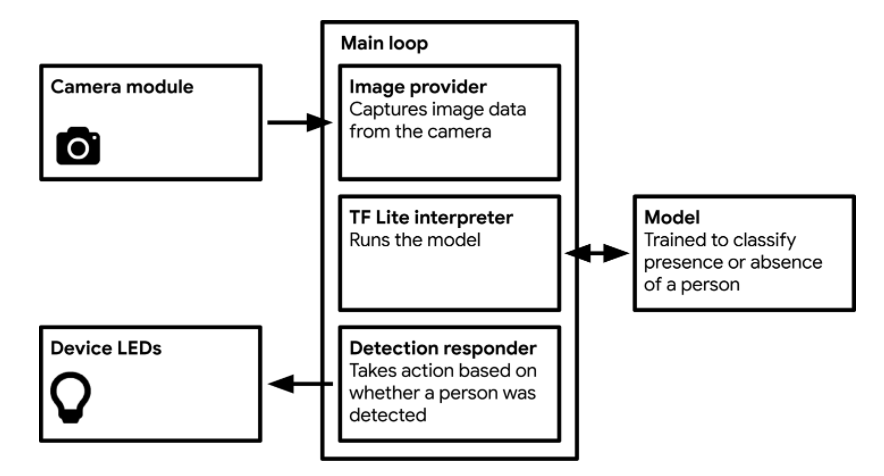
\includegraphics[width=0.9\textwidth]{Images/Arduino/tfLiteAblauf}
%	\caption{Diagram of the components of our person detection application}\label{tflite:Ablauf}
%\end{figure}
%
%Wie wir bereits erwähnt haben, ist dies viel einfacher als die Wake-Word-Anwendung, da wir die Bilddaten direkt in das Modell übergeben können - es ist keine Vorverarbeitung erforderlich.
%
%Ein weiterer Aspekt, der die Dinge einfach hält, ist, dass wir die Ausgabe des Modells nicht mitteln. Unser Wake-Word-Modell wurde mehrmals pro Sekunde ausgeführt, so dass wir seine Ausgabe mitteln mussten, um ein stabiles Ergebnis zu erhalten. Unser Personenerkennungsmodell ist viel größer und braucht viel länger, um die Inferenz auszuführen. Das bedeutet, dass es keine Notwendigkeit gibt, seine Ausgabe zu mitteln.
%
%Der Code besteht aus fünf Hauptteilen:
%
%\textbf{Main loop}
%
%Wie die anderen Beispiele läuft auch unsere Anwendung in einer Endlosschleife. Da unser Modell jedoch viel größer und komplexer ist, dauert es länger, bis die Inferenz ausgeführt wird. Je nach Gerät können wir eine Inferenz alle paar Sekunden erwarten, anstatt mehrere Inferenzen pro Sekunde.
%
%\textbf{Image provider}
%
%Diese Komponente erfasst Bilddaten von der Kamera und schreibt sie in den Eingangstensor. Die Methoden zur Erfassung von Bildern variieren von Gerät zu Gerät, daher kann diese Komponente überschrieben und angepasst werden.
%
%\textbf{TensorFlow Lite interpreter}
%
%Der Interpreter führt das TensorFlow Lite Modell aus und transformiert das Eingabebild in einen Satz von Wahrscheinlichkeiten.
%
%\textbf{Modell}
%
%Das Modell wird als Datenarray eingebunden und vom Interpreter ausgeführt. Mit 250 KB ist dieses Modell unangemessen groß, um es an das TensorFlow GitHub Repository zu übergeben. Aus diesem Grund wird es vom Makefile heruntergeladen, wenn das Projekt gebaut wird. Wenn Sie einen Blick darauf werfen wollen, können Sie es selbst unter \FILE{tf\_lite\_micro\_person\_data\_grayscale.zip} herunterladen.
%
%\textbf{Detection responder}
%
%
%Der Erkennungsresponder nimmt die vom Modell ausgegebenen Wahrscheinlichkeiten und verwendet die Ausgabefähigkeiten des Geräts, um sie anzuzeigen. Wir können ihn für verschiedene Gerätetypen überschreiben. In unserem Beispielcode leuchtet eine LED auf, aber Sie können ihn so erweitern, dass er so ziemlich alles tun kann.
%
%Um ein Gefühl dafür zu bekommen, wie diese Teile zusammenpassen, werfen wir einen Blick auf ihre Tests.
%
%\textbf{Durch die Tests gehen}
%
%Diese Anwendung ist schön einfach, da es nur ein paar Tests zu durchlaufen gibt. Sie können sie alle im GitHub-Repository finden:
%
%\FILE{person\_detection\_test.cc}
%
%Zeigt, wie eine Inferenz auf ein Array, das ein einzelnes Bild repräsentiert, ausgeführt werden kann
%
%\FILE{image\_provider\_test.cc}
%
%
%Zeigt, wie Sie den Bildanbieter verwenden, um ein Bild aufzunehmen
%
%\FILE{detection\_responder\_test.cc}
%
%Zeigt, wie der Erkennungsresponder verwendet wird, um die Ergebnisse der Erkennung auszugeben.
%
%Beginnen wir mit der Untersuchung von \FILE{person\_detection\_test.cc}, um zu sehen, wie die Inferenz auf Bilddaten ausgeführt wird. Da dies das dritte Beispiel ist, das wir durchlaufen haben, sollte Ihnen dieser Code ziemlich vertraut vorkommen. Sie sind auf dem besten Weg, ein eingebetteter ML-Entwickler zu werden!
%
%\textbf{Der Grundablauf}
%
%Beginnen wir mit der Datei \FILE{Person\_detection\_test.cc}. Wir beginnen damit, dass wir die Ops hineinziehen, die unser Modell benötigen wird:
%
%\begin{code}
%	
%	
%	%\lstinputlisting[firstline=1,lastline=136,firstnumber=10,language=c++]{../Code/Nano33BLESense/person_detection/person_detection_test.cc}    
%	
%	\begin{lstlisting}
%		namespace tflite {
%			namespace ops {
%				namespace micro {
%					TfLiteRegistration* Register_DEPTHWISE_CONV_2D();
%					TfLiteRegistration* Register_CONV_2D();
%					TfLiteRegistration* Register_AVERAGE_POOL_2D();
%				}  // namespace micro
%			}  // namespace ops
%		}  // namespace tflite
%	\end{lstlisting}
%\end{code}
%
%
%Als nächstes definieren wir eine Tensor-Arena, die für das Modell angemessen groß ist. Wie üblich wurde diese Zahl durch Versuch und Irrtum ermittelt:
%
%
%\begin{code}
%	\begin{lstlisting}
%		const int tensor_arena_size = 70 * 1024;
%		uint8_t tensor_arena[tensor_arena_size];
%	\end{lstlisting}
%\end{code}
%
%Anschließend führen wir die typischen Einrichtungsarbeiten durch, um den Interpreter einsatzbereit zu machen, wozu auch die Registrierung der erforderlichen Ops mit dem \PYTHON{MicroMutableOpResolver} gehört:
%
%\begin{code}
%	\begin{lstlisting}
%		// Set up logging.
%		tflite::MicroErrorReporter micro_error_reporter;
%		tflite::ErrorReporter* error_reporter = &micro_error_reporter;
%		
%		// Map the model into a usable data structure. This doesn't involve any
%		// copying or parsing, it's a very lightweight operation.
%		const tflite::Model* model = ::tflite::GetModel(g_person_detect_model_data);
%		if (model->version() != TFLITE_SCHEMA_VERSION) {
%			error_reporter->Report(
%			"Model provided is schema version %d not equal "
%			"to supported version %d.\n",
%			model->version(), TFLITE_SCHEMA_VERSION);
%		}
%		
%		// Pull in only the operation implementations we need.
%		tflite::MicroMutableOpResolver micro_mutable_op_resolver;
%		micro_mutable_op_resolver.AddBuiltin(
%		tflite::BuiltinOperator_DEPTHWISE_CONV_2D,
%		tflite::ops::micro::Register_DEPTHWISE_CONV_2D());
%		micro_mutable_op_resolver.AddBuiltin(tflite::BuiltinOperator_CONV_2D,
%		tflite::ops::micro::Register_CONV_2D());
%		micro_mutable_op_resolver.AddBuiltin(
%		tflite::BuiltinOperator_AVERAGE_POOL_2D,
%		tflite::ops::micro::Register_AVERAGE_POOL_2D());
%		
%		// Build an interpreter to run the model with.
%		tflite::MicroInterpreter interpreter(model, micro_mutable_op_resolver,
%		tensor_arena, tensor_arena_size,
%		error_reporter);
%		interpreter.AllocateTensors();
%	\end{lstlisting}
%\end{code}
%
%Unser nächster Schritt ist die Überprüfung des Eingabetensors. Wir prüfen, ob er die erwartete Anzahl von Dimensionen hat und ob seine Dimensionen angemessen dimensioniert sind:
%
%\begin{code}
%	\begin{lstlisting}
%		// Get information about the memory area to use for the model's input.
%		TfLiteTensor* input = interpreter.input(0);
%		
%		// Make sure the input has the properties we expect.
%		TF_LITE_MICRO_EXPECT_NE(nullptr, input);
%		TF_LITE_MICRO_EXPECT_EQ(4, input->dims->size);
%		TF_LITE_MICRO_EXPECT_EQ(1, input->dims->data[0]);
%		TF_LITE_MICRO_EXPECT_EQ(kNumRows, input->dims->data[1]);
%		TF_LITE_MICRO_EXPECT_EQ(kNumCols, input->dims->data[2]);
%		TF_LITE_MICRO_EXPECT_EQ(kNumChannels, input->dims->data[3]);
%		TF_LITE_MICRO_EXPECT_EQ(kTfLiteUInt8, input->type);
%	\end{lstlisting}
%\end{code}
%
%Daraus können wir erkennen, dass die Eingabe technisch gesehen ein 5D-Tensor ist. Die erste Dimension ist nur ein Wrapper, der ein einzelnes Element enthält. Die folgenden zwei Dimensionen stellen die Zeilen und Spalten der Pixel des Bildes dar. Die letzte Dimension enthält die Anzahl der Farbkanäle, die zur Darstellung jedes Pixels verwendet werden.
%
%Die Konstanten, die die erwarteten Dimensionen angeben, \PYTHON{kNumRows}, \PYTHON{kNumCols} und \PYTHON{kNumChannels}, sind in \FILE{model\_settings.h} definiert. Sie sehen folgendermaßen aus:
%
%\begin{code}
%	\begin{lstlisting}
%		constexpr int kNumCols = 96;
%		constexpr int kNumRows = 96;
%		constexpr int kNumChannels = 1;
%	\end{lstlisting}
%\end{code}
%
%Wie Sie sehen können, wird erwartet, dass das Modell eine Bitmap mit $96 \times 96$ Pixeln akzeptiert. Das Bild wird in Graustufen dargestellt, mit einem Farbkanal für jedes Pixel.
%
%Als nächstes im Code kopieren wir ein Testbild in den Eingangstensor mit einer einfachen for-Schleife:
%
%\begin{code}
%	\begin{lstlisting}
%		// Copy an image with a person into the memory area used for the input.
%		const uint8_t* person_data = g_person_data;
%		for (int i = 0; i < input->bytes; ++i) {
%			input->data.uint8[i] = person_data[i];
%		}
%	\end{lstlisting}
%\end{code}
%
%Die Variable, die die Bilddaten speichert, \PYTHON{g\_person\_data}, wird in der Datei \FILE{person\_image\_data.h} definiert. Um zu vermeiden, dass dem Repository weitere große Dateien hinzugefügt werden, werden die Daten selbst zusammen mit dem Modell heruntergeladen, als Teil von \FILE{tf\_lite\_micro\_person\_data\_grayscale.zip}, wenn die Tests zum ersten Mal ausgeführt werden.
%
%Nachdem wir den Eingabetensor aufgefüllt haben, führen wir die Inferenz durch. Es ist so einfach wie immer:
%
%\begin{code}
%	\begin{lstlisting}
%		// Run the model on this input and make sure it succeeds.
%		TfLiteStatus invoke_status = interpreter.Invoke();
%		if (invoke_status != kTfLiteOk) {
%			error_reporter->Report("Invoke failed\n");
%		}
%		TF_LITE_MICRO_EXPECT_EQ(kTfLiteOk, invoke_status);
%	\end{lstlisting}
%\end{code}
%
%Wir überprüfen nun den Ausgangstensor, um sicherzustellen, dass er die erwartete Größe und Form hat:
%
%\begin{code}
%	\begin{lstlisting}
%		TfLiteTensor* output = interpreter.output(0);
%		TF_LITE_MICRO_EXPECT_EQ(4, output->dims->size);
%		TF_LITE_MICRO_EXPECT_EQ(1, output->dims->data[0]);
%		TF_LITE_MICRO_EXPECT_EQ(1, output->dims->data[1]);
%		TF_LITE_MICRO_EXPECT_EQ(1, output->dims->data[2]);
%		TF_LITE_MICRO_EXPECT_EQ(kCategoryCount, output->dims->data[3]);
%		TF_LITE_MICRO_EXPECT_EQ(kTfLiteUInt8, output->type);
%	\end{lstlisting}
%\end{code}
%
%Die Ausgabe des Modells hat vier Dimensionen. Die ersten drei sind nur Umhüllungen für die vierte, die ein Element für jede Kategorie enthält, für die das Modell trainiert wurde.
%
%Die Gesamtzahl der Kategorien ist als Konstante kCategoryCount verfügbar, die sich zusammen mit einigen anderen hilfreichen Werten in \FILE{model\_settings.h} befindet:
%
%\begin{code}
%	\begin{lstlisting}
%		constexpr int kCategoryCount = 3;
%		constexpr int kPersonIndex = 1;
%		constexpr int kNotAPersonIndex = 2;
%		extern const char* kCategoryLabels[kCategoryCount];
%	\end{lstlisting}
%\end{code}
%
%Wie \PYTHON{kCategoryCount} zeigt, gibt es drei Kategorien in der Ausgabe. Die erste ist zufällig eine unbenutzte Kategorie, die wir ignorieren können. Die Kategorie "Person" kommt an zweiter Stelle, wie wir an ihrem Index erkennen können, der in der Konstante \PYTHON{kPersonIndex} gespeichert ist. An dritter Stelle steht die Kategorie "keine Person", deren Index durch \PYTHON{kNotAPersonIndex} angezeigt wird.
%
%Es gibt auch ein Array von Kategoriebezeichnungen, kCategoryLabels, das in \FILE{model\_settings.cc} implementiert ist:
%
%\begin{code}
%	\begin{lstlisting}
%		const char* kCategoryLabels[kCategoryCount] = {
%			"unused",
%			"person",
%			"notperson",
%		};
%	\end{lstlisting}
%\end{code}
%
%
%
%\subsection{Extra Dimensions}
%
%Wie \PYTHON{kCategoryCount} zeigt, gibt es drei Kategorien in der Ausgabe. Die erste ist zufällig eine unbenutzte Kategorie, die wir ignorieren können. Die Kategorie "Person" kommt an zweiter Stelle, wie wir an ihrem Index erkennen können, der in der Konstante kPersonIndex gespeichert ist. An dritter Stelle steht die Kategorie "keine Person", deren Index durch kNotAPersonIndex angezeigt wird.
%
%Es gibt auch ein Array von Kategoriebezeichnungen, \PYTHON{kCategoryLabels}, das in \FILE{model\_settings.cc} implementiert ist:
%Wie \PYTHON{kCategoryCount} zeigt, gibt es drei Kategorien in der Ausgabe. Die erste ist zufällig eine unbenutzte Kategorie, die wir ignorieren können. Die Kategorie "Person" kommt an zweiter Stelle, wie wir an ihrem Index erkennen können, der in der Konstante \PYTHON{kPersonIndex} gespeichert ist. An dritter Stelle steht die Kategorie "keine Person", deren Index durch \PYTHON{kNotAPersonIndex} angezeigt wird.
%
%Es gibt auch ein Array von Kategoriebezeichnungen, \PYTHON{kCategoryLabels}, das in \FILE{model\_settings.cc} implementiert ist:
%
%\begin{code}
%	\begin{lstlisting}
%		uint8_t person_score = output->data.uint8[kPersonIndex];
%		uint8_t no_person_score = output->data.uint8[kNotAPersonIndex];
%		error_reporter->Report(
%		"person data.  person score: %d, no person score: %d\n", person_score,
%		no_person_score);
%		TF_LITE_MICRO_EXPECT_GT(person_score, no_person_score);
%	\end{lstlisting}
%\end{code}
%
%Da der einzige Dateninhalt des Ausgabetensors die drei \PYTHON{uint8}-Werte sind, die die Klassenwerte darstellen, wobei der erste unbenutzt ist, können wir direkt auf die Werte zugreifen, indem wir \PYTHON{output->data.uint8[kPersonIndex]} und \PYTHON{output->data.uint8[kNotAPersonIndex]} verwenden. Als uint8-Typen haben sie einen Minimalwert von 0 und einen Maximalwert von 255.
%
%
%
%
%
%\subsection{NOTE}
%
%Wenn die Werte für "Person" und "keine Person" ähnlich sind, kann dies bedeuten, dass das Modell nicht sehr sicher in seiner Vorhersage ist. In diesem Fall können Sie das Ergebnis als nicht schlüssig betrachten.
%
%Als nächstes testen wir auf ein Bild ohne Person, das von \PYTHON{g\_no\_person\_data} gehalten wird:
%
%
%\begin{code}
%	\begin{lstlisting}
%		const uint8_t* no_person_data = g_no_person_data;
%		for (int i = 0; i < input->bytes; ++i) {
%			input->data.uint8[i] = no_person_data[i];
%		}
%	\end{lstlisting}
%\end{code}
%
%
%Nachdem die Inferenz gelaufen ist, behaupten wir dann, dass der Wert "keine Person" höher ist:
%
%\begin{code}
%	\begin{lstlisting}
%		person_score = output->data.uint8[kPersonIndex];
%		no_person_score = output->data.uint8[kNotAPersonIndex];
%		error_reporter->Report(
%		"no person data.  person score: %d, no person score: %d\n", person_score,
%		no_person_score);
%		TF_LITE_MICRO_EXPECT_GT(no_person_score, person_score);
%	\end{lstlisting}
%\end{code}
%
%Wie Sie sehen können, geht hier nichts Ausgefallenes vor sich. Wir geben zwar Bilder anstelle von Skalaren oder Spektrogrammen ein, aber der Prozess der Inferenz ist ähnlich zu dem, was wir zuvor gesehen haben.
%
%Das Ausführen des Tests ist ähnlich einfach. Geben Sie einfach den folgenden Befehl aus dem Stammverzeichnis des TensorFlow-Repositorys ein:
%
%\begin{code}
%	\begin{lstlisting}
%		make -f tensorflow/lite/micro/tools/make/Makefile \
%		test_person_detection_test
%	\end{lstlisting}
%\end{code}
%
%Wenn der Test das erste Mal ausgeführt wird, werden das Modell und die Bilddaten heruntergeladen. Wenn Sie einen Blick auf die heruntergeladenen Dateien werfen möchten, finden Sie diese in \FILE{tensorflow/lite/micro/tools/make/downloads/person\_model\_grayscale}. Siehe \url{../Code/Nano33BLESense/person_detection_int8}. Achtung ist eine C-Datei.
%
%Als Nächstes schauen wir uns die Schnittstelle für den Bildanbieter an.
%
%
%
%\subsection{The Image Provider}
%
%Der Image-Provider ist dafür verantwortlich, Daten von der Kamera abzugreifen und sie in einem Format zurückzugeben, das für das Schreiben in den Eingabetensor des Modells geeignet ist. Die Datei \FILE{image\_provider.h} definiert seine Schnittstelle:
%
%\begin{code}
%	\begin{lstlisting}
%		TfLiteStatus GetImage(tflite::ErrorReporter* error_reporter, int image_width,
%		int image_height, int channels, uint8_t* image_data);
%	\end{lstlisting}
%\end{code}
%
%Da die eigentliche Implementierung plattformspezifisch ist, gibt es eine Referenzimplementierung in \FILE{person\_detection/image\_provider.cc}, die Dummy-Daten zurückgibt.
%
%Der Test in \FILE{image\_provider\_test.cc} ruft diese Referenzimplementierung auf, um zu zeigen, wie sie verwendet wird. Als erstes müssen wir ein Array erstellen, das die Bilddaten enthält. Dies geschieht in der folgenden Zeile:
%
%\begin{code}
%	\begin{lstlisting}
%		uint8_t image_data[kMaxImageSize];
%	\end{lstlisting}
%\end{code}
%
%Die Konstante \PYTHON{kMaxImageSize} stammt aus unserem alten Freund, \FILE{model\_settings.h}.
%
%Nachdem wir dieses Array eingerichtet haben, können wir die Funktion \PYTHON{GetImage()} aufrufen, um ein Bild von der Kamera zu erfassen:
%
%\begin{code}
%	\begin{lstlisting}
%		TfLiteStatus get_status =
%		GetImage(error_reporter, kNumCols, kNumRows, kNumChannels, image_data);
%		TF_LITE_MICRO_EXPECT_EQ(kTfLiteOk, get_status);
%		TF_LITE_MICRO_EXPECT_NE(image_data, nullptr);
%	\end{lstlisting}
%\end{code}
%
%Wir rufen sie mit einer ErrorReporter-Instanz auf, mit der Anzahl der gewünschten Spalten, Zeilen und Kanäle und mit einem Zeiger auf unser Array \PYTHON{image\_data}. Die Funktion wird die Bilddaten in dieses Array schreiben. Wir können den Rückgabewert der Funktion überprüfen, um festzustellen, ob der Erfassungsprozess erfolgreich war; er wird auf \PYTHON{kTfLiteError} gesetzt, wenn es ein Problem gibt, oder andernfalls auf \PYTHON{kTfLiteOk}.
%
%Schließlich geht der Test durch die zurückgegebenen Daten, um zu zeigen, dass alle Speicherplätze lesbar sind. Auch wenn das Bild technisch gesehen Zeilen, Spalten und Kanäle hat, werden die Daten in der Praxis in ein 1D-Array gepresst:
%
%\begin{code}
%	\begin{lstlisting}
%		uint32_t total = 0;
%		for (int i = 0; i < kMaxImageSize; ++i) {
%			total += image_data[i];
%		}
%	\end{lstlisting}
%\end{code}
%
%Um diesen Test auszuführen, verwenden Sie den folgenden Befehl:
%
%\begin{code}
%	\begin{lstlisting}
%		make -f tensorflow/lite/micro/tools/make/Makefile \
%		test_image_provider_test
%	\end{lstlisting}
%\end{code}
%
%Wir werden die gerätespezifischen Implementierungen von \FILE{image\_provider.cc} später im Kapitel untersuchen; für den Moment wollen wir uns die Schnittstelle des Erkennungsresponders ansehen.
%
%\subsection{The Detection Responder}
%
%Unser letzter Test zeigt, wie der Erkennungsresponder verwendet wird. Dies ist der Code, der für die Übermittlung der Ergebnisse der Inferenz verantwortlich ist. Seine Schnittstelle ist in \FILE{detection\_responder.h} definiert, und der Test befindet sich in \FILE{detection\_responder\_test.cc}.
%
%Die Schnittstelle ist ziemlich einfach:
%
%\begin{code}
%	\begin{lstlisting}
%		void RespondToDetection(tflite::ErrorReporter* error_reporter,
%		uint8_t person_score, uint8_t no_person_score);
%	\end{lstlisting}
%\end{code}
%
%Wir rufen es einfach mit den Werten für die beiden Kategorien "Person" und "keine Person" auf, und es entscheidet, was von da an zu tun ist.
%
%Die Referenzimplementierung in \FILE{detection\_responder.cc} protokolliert nur diese Werte. Der Test in \FILE{detection\_responder\_test.cc} ruft die Funktion ein paar Mal auf:
%
%\begin{code}
%	\begin{lstlisting}
%		RespondToDetection(error_reporter, 100, 200);
%		RespondToDetection(error_reporter, 200, 100);
%	\end{lstlisting}
%\end{code}
%
%Um den Test auszuführen und die Ausgabe zu sehen, verwenden Sie den folgenden Befehl:
%
%\begin{code}
%	\begin{lstlisting}
%		make -f tensorflow/lite/micro/tools/make/Makefile \
%		test_detection_responder_test
%	\end{lstlisting}
%\end{code}
%
%Wir haben alle Tests und die Schnittstellen, die sie ausüben, erkundet. Lassen Sie uns nun das Programm selbst durchgehen.
%
%\subsection{Detecting People}
%
%Die Kernfunktionen der Anwendung befinden sich in DATEI{main\_functions.cc}. Sie sind kurz und bündig, und wir haben viel von ihrer Logik in den Tests gesehen.
%
%Zuerst holen wir uns alle Funktionen, die unser Modell benötigt:
%
%\begin{code}
%	\begin{lstlisting}
%		namespace tflite {
%			namespace ops {
%				namespace micro {
%					TfLiteRegistration* Register_DEPTHWISE_CONV_2D();
%					TfLiteRegistration* Register_CONV_2D();
%					TfLiteRegistration* Register_AVERAGE_POOL_2D();
%				}  // namespace micro
%			}  // namespace ops
%		}  // namespace tflite
%	\end{lstlisting}
%\end{code}
%
%Als nächstes deklarieren wir eine Reihe von Variablen, um die wichtigen beweglichen Teile zu halten:
%
%\begin{code}
%	\begin{lstlisting}
%		tflite::ErrorReporter* g_error_reporter = nullptr;
%		const tflite::Model* g_model = nullptr;
%		tflite::MicroInterpreter* g_interpreter = nullptr;
%		TfLiteTensor* g_input = nullptr;
%	\end{lstlisting}
%\end{code}
%
%Danach weisen wir etwas Arbeitsspeicher für Tensoroperationen zu:
%
%\begin{code}
%	\begin{lstlisting}
%		constexpr int g_tensor_arena_size = 70 * 1024;
%		static uint8_t tensor_arena[kTensorArenaSize];
%	\end{lstlisting}
%\end{code}
%
%In der Funktion \PYTHON{function}, die ausgeführt wird, bevor irgendetwas anderes passiert, erstellen wir einen Fehlerreporter, laden unser Modell, richten eine Interpreterinstanz ein und holen uns eine Referenz auf den Eingabetensor des Modells:
%
%\begin{code}
%	\begin{lstlisting}
%		void setup() {
%			// Set up logging.
%			static tflite::MicroErrorReporter micro_error_reporter;
%			g_error_reporter = &micro_error_reporter;
%			
%			// Map the model into a usable data structure. This doesn't involve any
%			// copying or parsing, it's a very lightweight operation.
%			g_model = tflite::GetModel(g_person_detect_model_data);
%			if (g_model->version() != TFLITE_SCHEMA_VERSION) {
%				g_error_reporter->Report(
%				"Model provided is schema version %d not equal "
%				"to supported version %d.",
%				g_model->version(), TFLITE_SCHEMA_VERSION);
%				return;
%			}
%			
%			// Pull in only the operation implementations we need.
%			static tflite::MicroMutableOpResolver micro_mutable_op_resolver;
%			micro_mutable_op_resolver.AddBuiltin(
%			tflite::BuiltinOperator_DEPTHWISE_CONV_2D,
%			tflite::ops::micro::Register_DEPTHWISE_CONV_2D());
%			micro_mutable_op_resolver.AddBuiltin(tflite::BuiltinOperator_CONV_2D,
%			tflite::ops::micro::Register_CONV_2D());
%			micro_mutable_op_resolver.AddBuiltin(
%			tflite::BuiltinOperator_AVERAGE_POOL_2D,
%			tflite::ops::micro::Register_AVERAGE_POOL_2D());
%			
%			// Build an interpreter to run the model with.
%			static tflite::MicroInterpreter static_interpreter(
%			model, micro_mutable_op_resolver, tensor_arena, kTensorArenaSize,
%			error_reporter);
%			interpreter = &static_interpreter;
%			
%			// Allocate memory from the tensor_arena for the model's tensors.
%			TfLiteStatus allocate_status = interpreter->AllocateTensors();
%			if (allocate_status != kTfLiteOk) {
%				error_reporter->Report("AllocateTensors() failed");
%				return;
%			}
%			
%			// Get information about the memory area to use for the model's input.
%			input = interpreter->input(0);
%		}
%	\end{lstlisting}
%\end{code}
%
%Der nächste Teil des Codes wird kontinuierlich in der Hauptschleife des Programms aufgerufen. Er holt sich zunächst ein Bild über den Image-Provider und übergibt eine Referenz auf den Input-Tensor, damit das Bild direkt dorthin geschrieben wird:
%
%\begin{code}
%	\begin{lstlisting}
%		void loop() {
%			// Get image from provider.
%			if (kTfLiteOk != GetImage(g_error_reporter, kNumCols, kNumRows, kNumChannels,
%			g_input->data.uint8)) {
%				g_error_reporter->Report("Image capture failed.");
%			}
%		\end{lstlisting}
%	\end{code}
%	
%	
%	Dann wird die Inferenz ausgeführt, der Ausgabetensor abgerufen und die "Person"- und "Keine Person"-Bewertungen daraus gelesen. Diese Scores werden an die Funktion \PYTHON{RespondToDetection()} des Erkennungsresponders übergeben:
%	
%	\begin{code}
%		\begin{lstlisting}
%			// Run the model on this input and make sure it succeeds.
%			if (kTfLiteOk != g_interpreter->Invoke()) {
%				g_error_reporter->Report("Invoke failed.");
%			}
%			
%			TfLiteTensor* output = g_interpreter->output(0);
%			
%			// Process the inference results.
%			uint8_t person_score = output->data.uint8[kPersonIndex];
%			uint8_t no_person_score = output->data.uint8[kNotAPersonIndex];
%			RespondToDetection(g_error_reporter, person_score, no_person_score);
%		}
%	\end{lstlisting}
%\end{code}
%
%Nachdem \PYTHON{RespondToDetection()} die Ausgabe der Ergebnisse beendet hat, kehrt die Funktion \PYTHON{loop()} zurück und ist bereit, von der Hauptschleife des Programms erneut aufgerufen zu werden.
%
%Die Schleife selbst wird in der Funktion \PYTHON{main()} des Programms definiert, die sich in main.cc befindet. Sie ruft die Funktion \PYTHON{setup()} einmal auf und ruft dann die Funktion \PYTHON{loop()} wiederholt und unendlich oft auf:
%
%\begin{code}
%	\begin{lstlisting}
%		int main(int argc, char* argv[]) {
%			setup();
%			while (true) {
%				loop();
%			}
%		}
%	\end{lstlisting}
%\end{code}
%
%Und das ist das gesamte Programm! Dieses Beispiel ist großartig, weil es zeigt, dass die Arbeit mit anspruchsvollen maschinellen Lernmodellen überraschend einfach sein kann. Das Modell enthält die gesamte Komplexität, und wir müssen es nur mit Daten füttern.
%
%Bevor wir weitermachen, können Sie das Programm lokal ausführen, um es auszuprobieren. Die Referenzimplementierung des Bildanbieters gibt nur Dummy-Daten zurück, so dass Sie keine aussagekräftigen Erkennungsergebnisse erhalten werden, aber Sie werden zumindest den Code bei der Arbeit sehen.
%
%Verwenden Sie zunächst diesen Befehl, um das Programm zu erstellen:
%
%\begin{code}
%	\begin{lstlisting}
%		make -f tensorflow/lite/micro/tools/make/Makefile person_detection
%	\end{lstlisting}
%\end{code}
%
%Sobald der Build abgeschlossen ist, können Sie das Beispiel mit dem folgenden Befehl ausführen:
%
%\begin{code}
%	\begin{lstlisting}
%		tensorflow/lite/micro/tools/make/gen/osx_x86_64/bin/ \
%		person_detection
%	\end{lstlisting}
%\end{code}
%
%Sie werden sehen, wie die Ausgabe des Programms vorbeiläuft, bis Sie es mit Strg-C beenden:
%
%\begin{code}
%	\begin{lstlisting}
%		person score:129 no person score 202
%		person score:129 no person score 202
%		person score:129 no person score 202
%		person score:129 no person score 202
%		person score:129 no person score 202
%		person score:129 no person score 202
%	\end{lstlisting}
%\end{code}
%
%Im nächsten Abschnitt gehen wir den gerätespezifischen Code durch, der Kamerabilder erfasst und die Ergebnisse auf jeder Plattform ausgibt. Wir zeigen auch, wie Sie diesen Code einsetzen und ausführen.
%
%\subsection{Einsatz auf Mikrocontrollern}
%
%In diesem Abschnitt stellen wir unseren Code auf zwei bekannten Geräten bereit:
%
%\begin{itemize}
%	\item  Arduino Nano 33 BLE Sense
%	\item SparkFun Edge
%\end{itemize}
%
%Diesmal gibt es einen großen Unterschied: Da keines dieser Geräte eine eingebaute Kamera hat, empfehlen wir Ihnen, ein Kameramodul für das jeweilige Gerät zu kaufen. Jedes Gerät hat seine eigene Implementierung von \FILE{image\_provider.cc}, die mit dem Kameramodul zusammenarbeitet, um Bilder zu erfassen. Es gibt auch einen gerätespezifischen Ausgabecode in \FILE{detection\_responder.cc}.
%
%Dies ist schön und einfach, so dass es eine ausgezeichnete Vorlage für die Erstellung Ihrer eigenen bildverarbeitungsbasierten ML-Anwendungen ist.
%
%Beginnen wir mit der Erkundung der Arduino-Implementierung.
%
%
%\subsection{Arduino}
%
%Als Arduino-Board hat das Arduino Nano 33 BLE Sense Zugriff auf ein riesiges Ökosystem kompatibler Hardware und Bibliotheken von Drittanbietern. Wir verwenden ein Kameramodul eines Drittanbieters, das für die Zusammenarbeit mit Arduino entwickelt wurde, zusammen mit einigen Arduino-Bibliotheken, die eine Schnittstelle zu unserem Kameramodul bilden und die von diesem ausgegebenen Daten sinnvoll nutzen.
%
%\subsection{Welches Kameramodul Sie kaufen sollten}
%
%Dieses Beispiel verwendet das Arducam Mini 2MP Plus Kameramodul. Es lässt sich einfach an den Arduino Nano 33 BLE Sense anschließen und kann über die Stromversorgung des Arduino-Boards mit Strom versorgt werden. Es hat ein großes Objektiv und kann qualitativ hochwertige 2-Megapixel-Bilder aufnehmen - allerdings werden wir die integrierte Bildskalierungsfunktion verwenden, um eine kleinere Auflösung zu erhalten. Sie ist nicht besonders stromsparend, aber ihre hohe Bildqualität macht sie ideal für den Aufbau von Bildaufnahme-Applikationen, z. B. für die Aufnahme von Wildtieren.
%
%\subsection{Aufnehmen von Bildern mit dem Arduino}
%
%Wir verbinden das Arducam-Modul über eine Reihe von Pins mit dem Arduino-Board. Um Bilddaten zu erhalten, senden wir einen Befehl vom Arduino-Board an die Arducam, der sie anweist, ein Bild aufzunehmen. Das Arducam wird dies tun und das Bild in seinem internen Datenpuffer speichern. Anschließend senden wir weitere Befehle, die es uns ermöglichen, die Bilddaten aus dem internen Puffer der Arducam zu lesen und sie im Speicher des Arduino zu speichern. Um all dies zu tun, verwenden wir die offizielle Arducam-Bibliothek.
%
%Das Arducam-Kameramodul hat einen 2-Megapixel-Bildsensor, mit einer Auflösung von 1920 × 1080. Unser Personenerkennungsmodell hat eine Eingabegröße von nur 96 × 96, so dass wir nicht alle diese Daten benötigen. Tatsächlich hat der Arduino selbst nicht genug Speicher, um ein 2-Megapixel-Bild zu speichern, das mehrere Megabyte groß wäre.
%
%Glücklicherweise ist die Arducam-Hardware in der Lage, ihre Ausgabe auf eine viel kleinere Auflösung von 160 × 120 Pixel zu verkleinern. Wir können dies in unserem Code leicht auf 96 × 96 verkleinern, indem wir nur die zentralen 96 × 96 Pixel beibehalten. Erschwerend kommt hinzu, dass die verkleinerte Ausgabe der Arducam mit JPEG kodiert ist, einem gängigen Kompressionsformat für Bilder. Unser Modell benötigt ein Array von Pixeln, kein JPEG-codiertes Bild, was bedeutet, dass wir die Ausgabe der Arducam dekodieren müssen, bevor wir sie verwenden. Wir können dies mit einer Open-Source-Bibliothek tun.
%
%Unsere letzte Aufgabe besteht darin, die Farbbildausgabe der Arducam in Graustufen zu konvertieren, was unser Modell zur Personenerkennung erwartet. Wir werden die Graustufendaten in den Eingabetensor unseres Modells schreiben.
%
%Der Image-Provider ist in \FILE{arduino/image\_provider.cc} implementiert. Wir werden hier nicht jedes Detail erklären, da der Code spezifisch für das Arducam-Kameramodul ist. Gehen wir stattdessen Schritt für Schritt durch, was auf hoher Ebene passiert.
%
%Die Funktion \PYTHON{GetImage()} ist die Schnittstelle des Bildanbieters zur Außenwelt. Sie wird in der Hauptschleife unserer Anwendung aufgerufen, um einen Frame mit Bilddaten zu erhalten. Wenn sie das erste Mal aufgerufen wird, müssen wir die Kamera initialisieren. Dies geschieht mit einem Aufruf der Funktion \PYTHON{InitCamera()}, wie folgt:
%
%
%
%
%\begin{code}
%	\begin{lstlisting}
%		static bool g_is_camera_initialized = false;
%		if (!g_is_camera_initialized) {
%			TfLiteStatus init_status = InitCamera(error_reporter);
%			if (init_status != kTfLiteOk) {
%				error_reporter->Report("InitCamera failed");
%				return init_status;
%			}
%			g_is_camera_initialized = true;
%		}
%	\end{lstlisting}
%\end{code}
%
%Die Funktion \PYTHON{InitCamera()} ist weiter oben in \FILE{image\_provider.cc} definiert. Wir werden sie hier nicht durchgehen, da sie sehr gerätespezifisch ist, und wenn Sie sie in Ihrem eigenen Code verwenden möchten, können Sie sie einfach kopieren und einfügen. Es konfiguriert die Arduino-Hardware für die Kommunikation mit der Arducam und bestätigt dann, dass die Kommunikation funktioniert. Schließlich weist sie die Arducam an, 160 × 120-Pixel-JPEG-Bilder auszugeben.
%
%Die nächste Funktion, die von \PYTHON{GetImage()} aufgerufen wird, ist \PYTHON{PerformCapture()}:
%
%\begin{code}
%	\begin{lstlisting}
%		TfLiteStatus capture_status = PerformCapture(error_reporter);
%	\end{lstlisting}
%\end{code}
%
%Wir werden auch hier nicht ins Detail gehen. Es sendet lediglich einen Befehl an das Kameramodul, der es anweist, ein Bild aufzunehmen und die Bilddaten in seinem internen Puffer zu speichern. Dann wartet es auf die Bestätigung, dass ein Bild aufgenommen wurde. Zu diesem Zeitpunkt warten die Bilddaten im internen Puffer der Arducam, aber es gibt noch keine Bilddaten auf dem Arduino selbst.
%
%Die nächste Funktion, die wir aufrufen, ist \PYTHON{ReadData()}:
%
%\begin{code}
%	\begin{lstlisting}
%		TfLiteStatus read_data_status = ReadData(error_reporter);
%	\end{lstlisting}
%\end{code}
%
%Die Funktion \PYTHON{ReadData()} verwendet weitere Befehle, um die Bilddaten von der Arducam zu holen. Nachdem die Funktion ausgeführt wurde, wird die globale Variable \PYTHON{jpeg\_buffer} mit den von der Kamera abgerufenen JPEG-kodierten Bilddaten gefüllt.
%
%Wenn wir das JPEG-kodierte Bild haben, ist unser nächster Schritt, es in rohe Bilddaten zu dekodieren. Dies geschieht mit der Funktion \PYTHON{DecodeAndProcessImage()}:
%
%\begin{code}
%	\begin{lstlisting}
%		TfLiteStatus decode_status = DecodeAndProcessImage(
%		error_reporter, image_width, image_height, image_data);
%	\end{lstlisting}
%\end{code}
%
%Die Funktion verwendet eine Bibliothek namens \FILE{JPEGDecoder}, um die JPEG-Daten zu dekodieren und direkt in den Eingangstensor des Modells zu schreiben. Dabei beschneidet sie das Bild und verwirft einige der 160 × 120 Daten, so dass nur 96 × 96 Pixel übrig bleiben, etwa in der Mitte des Bildes. Außerdem wird die 16-Bit-Farbdarstellung des Bildes auf 8-Bit-Graustufen reduziert.
%
%Nachdem das Bild erfasst und im Eingabetensor gespeichert wurde, können wir die Inferenz ausführen. Als nächstes zeigen wir, wie die Ausgabe des Modells angezeigt wird
%
%\subsection{Reagieren auf Erkennungen am Arduino}
%
%Der Arduino Nano 33 BLE Sense verfügt über eine eingebaute RGB-LED, d. h. eine einzelne Komponente, die unterschiedliche rote, grüne und blaue LEDs enthält, die Sie separat steuern können. Bei der Implementierung des Erkennungsresponders blinkt die blaue LED jedes Mal, wenn eine Inferenz ausgeführt wird. Wenn eine Person erkannt wird, leuchtet die grüne LED; wenn eine Person nicht erkannt wird, leuchtet die rote LED.
%
%Die Implementierung befindet sich in \FILE{arduino/detection\_responder.cc}. Lassen Sie uns kurz durchgehen.
%
%Die Funktion \PYTHON{RespondToDetection()} akzeptiert zwei Wertungen, eine für die Kategorie "Person" und die andere für "keine Person". Beim ersten Aufruf werden die blauen, grünen und gelben LEDs für die Ausgabe eingerichtet:
%
%\begin{code}
%	\begin{lstlisting}
%		void RespondToDetection(tflite::ErrorReporter* error_reporter,
%		uint8_t person_score, uint8_t no_person_score) {
%			static bool is_initialized = false;
%			if (!is_initialized) {
%				pinMode(led_green, OUTPUT);
%				pinMode(led_blue, OUTPUT);
%				is_initialized = true;
%			}
%		\end{lstlisting}
%	\end{code}
%	
%	Um anzuzeigen, dass eine Inferenz gerade abgeschlossen wurde, schalten wir als nächstes alle LEDs aus und lassen dann die blaue LED ganz kurz aufblinken:
%	
%	\begin{code}
%		\begin{lstlisting}
%			// Note: The RGB LEDs on the Arduino Nano 33 BLE
%			// Sense are on when the pin is LOW, off when HIGH.
%			
%			// Switch the person/not person LEDs off
%			digitalWrite(led_green, HIGH);
%			digitalWrite(led_red, HIGH);
%			
%			// Flash the blue LED after every inference.
%			digitalWrite(led_blue, LOW);
%			delay(100);
%			digitalWrite(led_blue, HIGH);
%		\end{lstlisting}
%	\end{code}
%	
%	Sie werden feststellen, dass diese LEDs im Gegensatz zu den eingebauten LEDs des Arduinos mit LOW eingeschaltet und mit HIGH ausgeschaltet werden. Das liegt einfach daran, wie die LEDs mit der Platine verbunden sind.
%	
%	Als Nächstes schalten wir die entsprechenden LEDs ein und aus, je nachdem, welcher Kategorienwert höher ist:
%	
%	\begin{code}
%		\begin{lstlisting}
%			// Switch on the green LED when a person is detected,
%			// the red when no person is detected
%			if (person_score > no_person_score) {
%				digitalWrite(led_green, LOW);
%				digitalWrite(led_red, HIGH);
%			} else {
%				digitalWrite(led_green, HIGH);
%				digitalWrite(led_red, LOW);
%			}
%		\end{lstlisting}
%	\end{code}
%	
%	Schließlich verwenden wir die Instanz \PYTHON{error\_reporter}, um die Ergebnisse auf der seriellen Schnittstelle auszugeben:
%	
%	\begin{code}
%		\begin{lstlisting}
%			error_reporter->Report("Person score: %d No person score: %d", person_score,
%			no_person_score);
%		}
%	\end{lstlisting}
%\end{code}
%
%Und das war's! Der Kern der Funktion ist eine einfache if-Anweisung, und Sie könnten leicht eine ähnliche Logik verwenden, um andere Arten von Ausgaben zu steuern. Es hat etwas sehr Spannendes, wenn eine so komplexe visuelle Eingabe in eine einzige boolesche Ausgabe umgewandelt wird: "Person" oder "keine Person".
%
%\subsection{Ausführen des Beispiels}
%
%Die Ausführung dieses Beispiels ist ein wenig komplexer als unsere anderen Arduino-Beispiele, da wir die Arducam mit dem Arduino-Board verbinden müssen. Außerdem müssen wir die Bibliotheken installieren und konfigurieren, die die Schnittstelle zur Arducam bilden und deren JPEG-Ausgabe dekodieren. Aber keine Sorge, es ist trotzdem sehr einfach!
%
%Um dieses Beispiel zu implementieren, benötigen wir Folgendes:
%
%\begin{itemize}
%	\item An Arduino Nano 33 BLE Sense board
%	\item An Arducam Mini 2MP Plus
%	\item Jumper cables (and optionally a breadboard)
%	\item A micro-USB cable
%	\item The Arduino IDE
%\end{itemize}
%
%Unsere erste Aufgabe besteht darin, das Arducam mit Hilfe von Jumper-Kabeln an den Arduino anzuschließen. Dies ist kein Elektronikbuch, daher werden wir nicht auf die Details der Verwendung der Kabel eingehen. Stattdessen zeigt Tabelle~\ref{ArducamPins}, wie die Pins angeschlossen werden sollten. Die Pins sind auf jedem Gerät beschriftet.
%
%\begin{table}
%	\centering
%	
%	\begin{tabular}{ll}    
%		Arducam pin & Arduino pin \\
%		CS   & D7 (unlabeled, immediately to the right of D6) \\
%		MOSI & D11 \\
%		MISO & D12 \\
%		SCK  & D13 \\
%		GND  & GND (either pin marked GND is fine) \\
%		VCC  & 3.3 V \\
%		SDA  & A4 \\
%		SCL  & A5 \\
%	\end{tabular}
%	\caption{ Arducam Mini 2MP Plus to Arduino Nano 33 BLE Sense connections}\label{ArducamPins}
%	
%\end{table}
%
%Nachdem Sie die Hardware eingerichtet haben, können Sie mit der Installation der Software fortfahren.
%
%\subsection{Tip}
%
%Es besteht immer die Möglichkeit, dass sich der Erstellungsprozess geändert hat, seit dieses Buch geschrieben wurde, also überprüfen Sie \FILE{README.md} auf die neuesten Anweisungen.
%
%Die Projekte in diesem Buch sind als Beispielcode in der TensorFlow Lite Arduino-Bibliothek verfügbar. Wenn Sie die Bibliothek noch nicht installiert haben, öffnen Sie die Arduino IDE und wählen Sie Bibliotheken verwalten aus dem Menü Werkzeuge. Suchen Sie im erscheinenden Fenster nach der Bibliothek mit dem Namen \FILE{Arduino\_TensorFlowLite} und installieren Sie sie. Sie sollten in der Lage sein, die neueste Version zu verwenden, aber wenn Sie auf Probleme stoßen, ist die Version, die mit diesem Buch getestet wurde, 1.14-ALPHA.
%
%\subsection{Bemerkung}
%
%Sie können die Bibliothek auch aus einer .zip-Datei installieren, die Sie entweder vom TensorFlow Lite Team herunterladen oder mit dem TensorFlow Lite for Microcontrollers Makefile selbst erzeugen können. Wenn Sie letzteres bevorzugen, lesen Sie Anhang A.
%
%Nachdem Sie die Bibliothek installiert haben, erscheint das Beispiel \FILE{person\_detection} im Menü File unter \FILE{Examples->Arduino\_TensorFlowLite}, wie in Abbildung~\ref{tinyML9-2} gezeigt.
%
%\begin{figure}
%	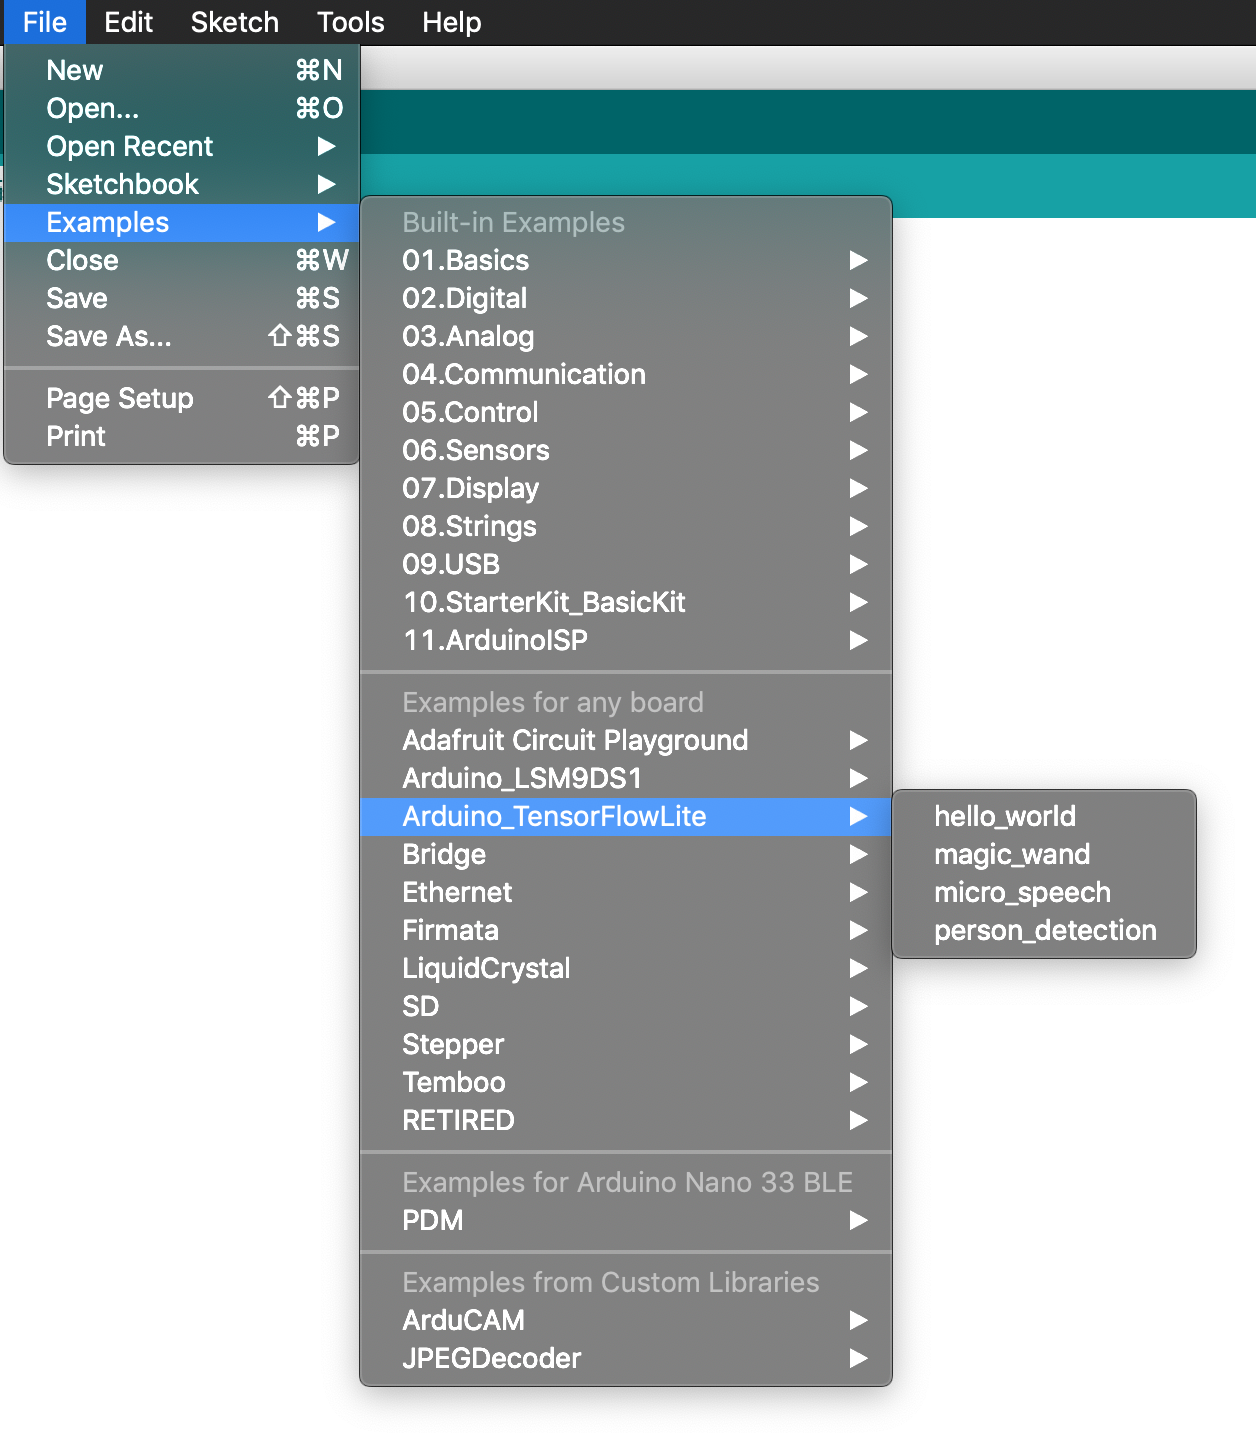
\includegraphics{Images/Arduino/tinyML9-2}
%	\caption{Screenshot des Menüs 'Examples'}\label{tinyML9-2}
%\end{figure}
%
%
%
%Klicken Sie auf \FILE{\glqq person\_detection\grqq}, um das Beispiel zu laden. Es erscheint ein neues Fenster mit einer Registerkarte für jede der Quelldateien. Die Datei in der ersten Registerkarte, \FILE{person\_detection}, entspricht der Datei \FILE{main\_functions.cc}, die wir zuvor durchgelesen haben.
%
%\subsection{Bemerkung}
%
%"Das Ausführen des Beispiels" hat bereits die Struktur des Arduino-Beispiels erklärt, daher werden wir es hier nicht noch einmal behandeln.
%
%Zusätzlich zur TensorFlow-Bibliothek müssen wir zwei weitere Bibliotheken installieren:
%
%\begin{enumerate}
%	\item Die Bibliothek \FILE{Arducam}, damit unser Code mit der Hardware interagieren kann
%	\item Die Bibliothek \FILE{JPEGDecoder}, damit wir JPEG-kodierte Bilder dekodieren können
%\end{enumerate}
%
%Die Arducam-Arduino-Bibliothek ist auf GitHub verfügbar. Um sie zu installieren, laden Sie das Repository herunter oder klonen Sie es. Kopieren Sie anschließend das Unterverzeichnis \FILE{ArduCAM} in Ihr Verzeichnis \FILE{Arduino/libraries}. Um das Bibliotheksverzeichnis auf Ihrem Rechner zu finden, überprüfen Sie den Sketchbook-Speicherort im Voreinstellungsfenster der Arduino IDE.
%
%Nachdem Sie die Bibliothek heruntergeladen haben, müssen Sie eine ihrer Dateien bearbeiten, um sicherzustellen, dass sie für die Arducam Mini 2MP Plus konfiguriert ist. Öffnen Sie dazu \FILE{Arduino/libraries/ArduCAM/memorysaver.h}.
%
%Sie sollten eine Reihe von \PYTHON{\#define}-Anweisungen aufgelistet sehen. Stellen Sie sicher, dass sie alle auskommentiert sind, außer \PYTHON{\#define OV2640\_MINI\_2MP\_PLUS}, wie hier gezeigt:
%
%\begin{code}
%	\begin{lstlisting}
%		//Step 1: select the hardware platform, only one at a time
%		//#define OV2640_MINI_2MP
%		//#define OV3640_MINI_3MP
%		//#define OV5642_MINI_5MP
%		//#define OV5642_MINI_5MP_BIT_ROTATION_FIXED
%		#define OV2640_MINI_2MP_PLUS
%		//#define OV5642_MINI_5MP_PLUS
%		//#define OV5640_MINI_5MP_PLUS
%	\end{lstlisting}
%\end{code}
%
%Nachdem Sie die Datei gespeichert haben, sind Sie mit der Konfiguration der Arducam-Bibliothek fertig.
%
%\subsection{Tip}
%
%Das Beispiel wurde mit \SHELL{Commit \#e216049} der Arducam-Bibliothek entwickelt. Wenn Sie Probleme mit der Bibliothek haben, können Sie versuchen, diesen speziellen Commit herunterzuladen, um sicherzustellen, dass Sie genau denselben Code verwenden.
%
%Der nächste Schritt ist die Installation der Bibliothek \FILE{JPEGDecoder}. Sie können dies aus der Arduino-IDE heraus tun. Wählen Sie im Menü "Tools" die Option "Manage Libraries" und suchen Sie nach \FILE{JPEGDecoder}. Sie sollten die Version 1.8.0 der Bibliothek installieren.
%
%Nachdem Sie die Bibliothek installiert haben, müssen Sie sie konfigurieren, um einige optionale Komponenten zu deaktivieren, die nicht mit dem Arduino Nano 33 BLE Sense kompatibel sind. Öffnen Sie \FILE{Arduino/libraries/JPEGDecoder/src/User\_Config.h} und stellen Sie sicher, dass sowohl \PYTHON{\#define LOAD\_SD\_LIBRARY} als auch \PYTHON{\#define LOAD\_SDFAT\_LIBRAR} auskommentiert sind, wie in diesem Auszug aus der Datei gezeigt:
%
%\begin{code}
%	\begin{lstlisting}
%		// Comment out the next #defines if you are not using an SD Card to store
%		// the JPEGs
%		// Commenting out the line is NOT essential but will save some FLASH space if
%		// SD Card access is not needed. Note: use of SdFat is currently untested!
%		
%		//#define LOAD_SD_LIBRARY // Default SD Card library
%		//#define LOAD_SDFAT_LIBRARY // Use SdFat library instead, so SD Card SPI can
%		// be bit bashed
%	\end{lstlisting}
%\end{code}
%
%Nachdem Sie die Datei gespeichert haben, ist die Installation der Bibliotheken abgeschlossen. Sie sind nun bereit, die Anwendung zur Personenerkennung auszuführen!
%
%Schließen Sie zunächst Ihr Arduino-Gerät über USB an. Vergewissern Sie sich, dass der richtige Gerätetyp in der Dropdown-Liste "Board" im Menü "Tools" ausgewählt ist, wie in Abbildung~\ref{tinyML9-3} gezeigt.
%
%\begin{figure}
%	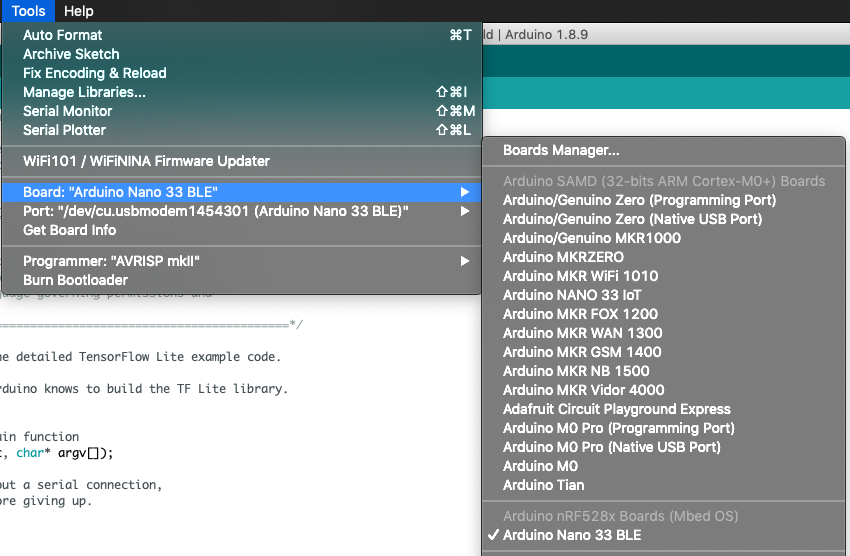
\includegraphics{Images/Arduino/tinyML9-3}
%	\caption{Screenshot of the 'Board' dropdown}\label{tinyML9-3}
%\end{figure}
%
%
%Wenn der Name Ihres Geräts nicht in der Liste erscheint, müssen Sie sein Support-Paket installieren. Klicken Sie dazu auf Boards Manager. Suchen Sie in dem daraufhin angezeigten Fenster nach Ihrem Gerät und installieren Sie die neueste Version des entsprechenden Support-Pakets.
%
%Vergewissern Sie sich auch im Menü Tools, dass der Anschluss des Geräts in der Dropdown-Liste Port ausgewählt ist, wie in Abbildung~\ref{tinyML9-4} gezeigt.
%
%\begin{figure}
%	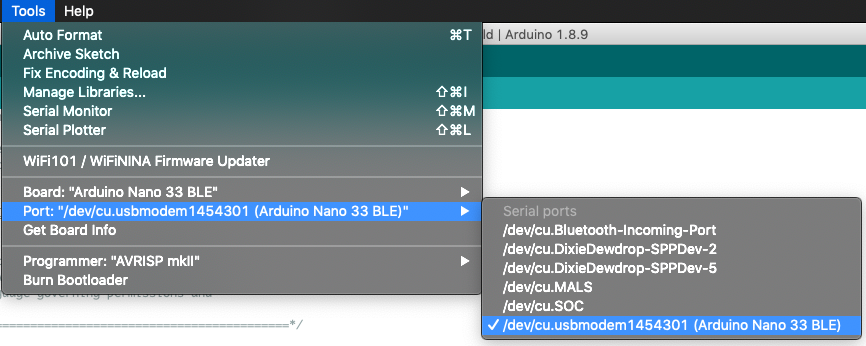
\includegraphics{Images/Arduino/tinyML9-4}
%	\caption{Screenshot of the 'Port' dropdown}\label{tinyML9-4}
%\end{figure}
%
%
%Klicken Sie schließlich im Arduino-Fenster auf die Schaltfläche "Hochladen" (in Abbildung~\ref{tinyML9-4} weiß hervorgehoben), um den Code zu kompilieren und auf Ihr Arduino-Gerät hochzuladen.
%
%
%\begin{figure}
%	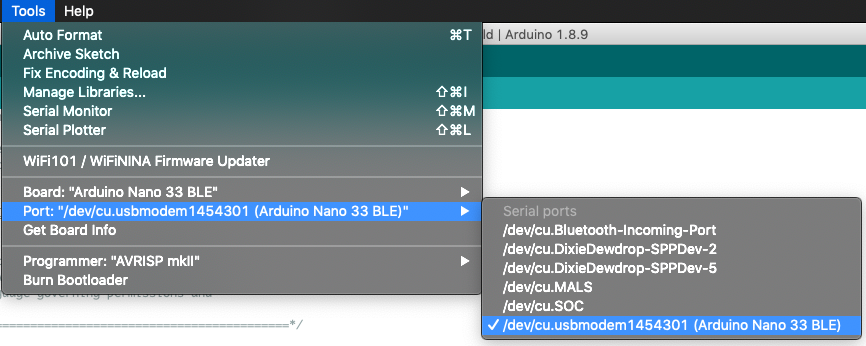
\includegraphics{Images/Arduino/tinyML9-4}
%	\caption{Screenshot of the upload button}\label{tinyML9-4}
%\end{figure}
%
%Sobald der Upload erfolgreich abgeschlossen ist, wird das Programm ausgeführt.
%
%Um es zu testen, beginnen Sie damit, die Kamera des Geräts auf etwas zu richten, das definitiv keine Person ist oder nur das Objektiv verdeckt. Wenn die blaue LED das nächste Mal blinkt, nimmt das Gerät ein Bild von der Kamera auf und beginnt, die Inferenz auszuführen. Da das Bildverarbeitungsmodell, das wir für die Personenerkennung verwenden, relativ groß ist, wird die Inferenz sehr lange dauern - etwa 19 Sekunden zum Zeitpunkt des Schreibens, obwohl es möglich ist, dass TensorFlow Lite seitdem schneller geworden ist.
%
%Wenn die Inferenz abgeschlossen ist, wird das Ergebnis in eine weitere leuchtende LED übersetzt. Sie haben die Kamera auf etwas gerichtet, das keine Person ist, also sollte die rote LED aufleuchten.
%
%Versuchen Sie nun, die Kamera des Geräts auf sich selbst zu richten! Wenn die blaue LED das nächste Mal blinkt, nimmt das Gerät ein weiteres Bild auf und beginnt, die Inferenz durchzuführen. Nach etwa 19 Sekunden sollte die grüne LED aufleuchten.
%
%Denken Sie daran, dass die Bilddaten vor jeder Inferenz als Schnappschuss aufgenommen werden, wenn die blaue LED blinkt. Das, worauf die Kamera in diesem Moment gerichtet ist, wird in das Modell eingespeist. Es spielt keine Rolle, worauf die Kamera gerichtet ist, bis das nächste Mal ein Bild aufgenommen wird, wenn die blaue LED wieder blinkt.
%
%Wenn Sie scheinbar falsche Ergebnisse erhalten, stellen Sie sicher, dass Sie sich in einer Umgebung mit guter Beleuchtung befinden. Sie sollten auch sicherstellen, dass die Kamera richtig ausgerichtet ist, mit den Stiften nach unten, so dass die Bilder, die sie aufnimmt, richtig herum sind - das Modell wurde nicht darauf trainiert, auf dem Kopf stehende Personen zu erkennen. Außerdem sollten Sie bedenken, dass es sich um ein winziges Modell handelt, bei dem die Genauigkeit gegen die geringe Größe eingetauscht wird. Es funktioniert sehr gut, aber es ist nicht immer zu 100 % genau.
%
%Sie können die Ergebnisse der Inferenz auch über den Arduino Serial Monitor sehen. Öffnen Sie dazu im Menü "Tools" den "Serial Monitor". Sie werden ein detailliertes Protokoll sehen, das zeigt, was passiert, während die Anwendung läuft. Es ist auch interessant, das Kästchen "Show timestamp" (Zeitstempel anzeigen) zu aktivieren, damit Sie sehen können, wie lange jeder Teil des Prozesses dauert:
%
%
%
%
%\begin{code}
%	\begin{lstlisting}
%		14:17:50.714 -> Starting capture
%		14:17:50.714 -> Image captured
%		14:17:50.784 -> Reading 3080 bytes from ArduCAM
%		14:17:50.887 -> Finished reading
%		14:17:50.887 -> Decoding JPEG and converting to greyscale
%		14:17:51.074 -> Image decoded and processed
%		14:18:09.710 -> Person score: 246 No person score: 66
%	\end{lstlisting}
%\end{code}
%
%Aus diesem Protokoll ist ersichtlich, dass das Erfassen und Lesen der Bilddaten vom Kameramodul ca. 170 ms, das Dekodieren des JPEGs und die Umwandlung in Graustufen 180 ms und die Durchführung der Inferenz 18,6 Sekunden dauerte.
%
%\subsection{Ausführung von Änderungen}
%
%Jetzt, wo Sie die Basisanwendung bereitgestellt haben, können Sie ein wenig herumspielen und einige Änderungen am Code vornehmen. Bearbeiten Sie einfach die Dateien in der Arduino-IDE und speichern Sie sie, und wiederholen Sie dann die vorherigen Anweisungen, um den geänderten Code auf dem Gerät einzusetzen.
%
%Hier sind ein paar Dinge, die Sie ausprobieren können:
%
%\begin{itemize}
%	\item Ändern Sie den Erkennungsresponder so, dass er mehrdeutige Eingaben ignoriert, bei denen es keinen großen Unterschied zwischen den Bewertungen "Person" und "keine Person" gibt.
%	\item Verwenden Sie die Ergebnisse der Personenerkennung, um andere Komponenten zu steuern, z. B. zusätzliche LEDs oder Servos.
%	\item Bauen Sie eine intelligente Sicherheitskamera, indem Sie Bilder speichern oder übertragen - aber nur solche, die eine Person enthalten.
%\end{itemize}
%
%
%
%
%
%
%
%
%
%
%
%
%
%
%
%
%
%
%
%
%
%\cite{Chowdhery:2019}
%
%
%\url{https://github.com/tensorflow/tensorflow/tree/master/tensorflow/lite/micro/examples/person\_detection}
%
%\subsection{Laufen auf Arduino}
%
%Die folgenden Anweisungen helfen Ihnen, dieses Beispiel zu erstellen und auf Arduino-Geräten einzusetzen.
%
%Das Beispiel wurde mit dem folgenden Gerät getestet:
%
%Arduino Nano 33 BLE Sense
%Sie benötigen außerdem das folgende Kameramodul:
%
%Arducam Mini 2MP Plus
%
%Hardware
%Schließen Sie die Pins der Arducam wie folgt an:
%
%\begin{tabular}{ll}
%	Arducam pin name & Arduino pin name \\ \hline
%	CS               & D7 (unlabelled, immediately to the right of D6) \\
%	MOSI             & D11 \\
%	MISO             & D12 \\
%	SCK              & D13 \\
%	GND              & GND (either pin marked GND is fine) \\
%	VCC              & 3.3 V \\
%	SDA              & A4 \\
%	SCL              & A5 \\
%\end{tabular}
%
%Installieren Sie die Bibliothek \FILE{Arduino\_TensorFlowLite}
%
%Laden Sie den aktuellen nächtlichen Build der Bibliothek herunter: \FILE{person\_detection.zip}
%
%Diese Beispielanwendung ist als Teil der offiziellen TensorFlow Lite Arduino-Bibliothek enthalten. Um sie zu installieren, öffnen Sie den Arduino Bibliotheksmanager in Tools -> Manage Libraries... und suchen Sie nach \FILE{Arduino\_TensorFlowLite}.
%
%\subsection{Installation anderer Bibliotheken}
%
%Zusätzlich zur TensorFlow-Bibliothek müssen Sie noch zwei weitere Bibliotheken installieren:
%
%Die Arducam-Bibliothek, damit unser Code mit der Hardware kommunizieren kann
%Die JPEGDecoder-Bibliothek, so dass wir JPEG-kodierte Bilder dekodieren können
%Die Arducam-Arduino-Bibliothek ist auf GitHub unter \url{https://github.com/ArduCAM/Arduino} verfügbar. Um sie zu installieren, laden Sie das Repository herunter oder klonen Sie es. Kopieren Sie anschließend das Unterverzeichnis ArduCAM in Ihr Arduino/libraries-Verzeichnis. Um dieses Verzeichnis auf Ihrem Rechner zu finden, überprüfen Sie den Sketchbook-Speicherort im Fenster "Einstellungen" der Arduino IDE.
%
%Nachdem Sie die Bibliothek heruntergeladen haben, müssen Sie eine ihrer Dateien bearbeiten, um sicherzustellen, dass sie für die Arducam Mini 2MP Plus konfiguriert ist. Öffnen Sie dazu die folgende Datei:
%
%\FILE{Arduino/libraries/ArduCAM/memorysaver.h}
%
%You'll see a bunch of \PYTHON{\#define} statements listed. Make sure that they are all commented out, except for \PYTHON{\#define OV2640\_MINI\_2MP\_PLUS}, as so:
%
%\begin{code}
%	\begin{lstlisting}
%		//Step 1: select the hardware platform, only one at a time
%		//#define OV2640_MINI_2MP
%		//#define OV3640_MINI_3MP
%		//#define OV5642_MINI_5MP
%		//#define OV5642_MINI_5MP_BIT_ROTATION_FIXED
%		#define OV2640_MINI_2MP_PLUS
%		//#define OV5642_MINI_5MP_PLUS
%		//#define OV5640_MINI_5MP_PLUS
%	\end{lstlisting}
%\end{code}
%
%Sobald Sie die Datei gespeichert haben, sind wir mit der Konfiguration der Arducam-Bibliothek fertig.
%
%Unser nächster Schritt ist die Installation der JPEGDecoder-Bibliothek. Wir können dies aus der Arduino-IDE heraus tun. Gehen Sie zunächst auf die Option "Manage Libraries..." im Menü "Tools" und suchen Sie nach JPEGDecoder. Sie sollten die Version 1.8.0 der Bibliothek installieren.
%
%Sobald die Bibliothek installiert ist, müssen wir sie konfigurieren, um einige optionale Komponenten zu deaktivieren, die nicht mit dem Arduino Nano 33 BLE Sense kompatibel sind. Öffnen Sie die folgende Datei:
%
%\FILE{Arduino/libraries/JPEGDecoder/src/User\_Config.h}
%
%Stellen Sie sicher, dass sowohl \PYTHON{\#define LOAD\_SD\_LIBRARY} als auch \PYTHON{\#define LOAD\_SDFAT\_LIBRARY} auskommentiert sind, wie in diesem Auszug aus der Datei gezeigt:
%
%
%\begin{code}
%	\begin{lstlisting}
%		// Comment out the next #defines if you are not using an SD Card to store the JPEGs
%		// Commenting out the line is NOT essential but will save some FLASH space if
%		// SD Card access is not needed. Note: use of SdFat is currently untested!
%		
%		//#define LOAD_SD_LIBRARY // Default SD Card library
%		//#define LOAD_SDFAT_LIBRARY // Use SdFat library instead, so SD Card SPI can be bit bashed-device, then build and upload the example.
%	\end{lstlisting}
%\end{code}
%
%
%
%Um die Kamera zu testen, beginnen Sie damit, die Kamera des Geräts auf etwas zu richten, das definitiv keine Person ist, oder sie einfach zu verdecken. Wenn die blaue LED das nächste Mal blinkt, erfasst das Gerät ein Bild von der Kamera und beginnt mit der Inferenz. Das Bildverarbeitungsmodell, das wir für die Personenerkennung verwenden, ist relativ groß, aber mit den cmsis-nn-Optimierungen dauert es nur etwa 800 ms, um das Modell auszuführen.
%
%Nach einem Moment wird das Ergebnis der Inferenz in das Aufleuchten einer weiteren LED umgesetzt. Da Sie die Kamera auf etwas gerichtet haben, das keine Person ist, sollte die rote LED aufleuchten.
%
%Versuchen Sie nun, die Kamera des Geräts auf sich selbst zu richten! Wenn die blaue LED das nächste Mal blinkt, nimmt das Gerät ein weiteres Bild auf und beginnt, die Inferenz durchzuführen. Nach einer kurzen Pause sollte die grüne LED aufleuchten!
%
%Denken Sie daran, dass die Bilddaten vor jeder Inferenz als Schnappschuss aufgenommen werden, wenn die blaue LED blinkt. Das, worauf die Kamera in diesem Moment gerichtet ist, wird in das Modell eingespeist. Es spielt keine Rolle, wohin die Kamera gerichtet ist, bis das nächste Mal ein Bild aufgenommen wird, wenn die blaue LED wieder blinkt.
%
%Wenn Sie scheinbar falsche Ergebnisse erhalten, stellen Sie sicher, dass Sie sich in einer Umgebung mit guter Beleuchtung befinden. Sie sollten auch sicherstellen, dass die Kamera richtig ausgerichtet ist, mit den Stiften nach unten, so dass die Bilder, die sie aufnimmt, richtig herum sind - das Modell wurde nicht darauf trainiert, auf dem Kopf stehende Personen zu erkennen! Außerdem sollte man bedenken, dass es sich um ein winziges Modell handelt, bei dem die Genauigkeit gegen die geringe Größe eingetauscht wird. Es funktioniert sehr gut, aber es ist nicht immer zu 100 % genau.
%
%Wir können die Ergebnisse der Inferenz auch über den Arduino Serial Monitor sehen. Dazu öffnen Sie den Serial Monitor aus dem Menü Tools. Sie werden ein detailliertes Protokoll dessen sehen, was passiert, während unsere Anwendung läuft. Es ist auch interessant, das Kontrollkästchen Zeitstempel anzeigen zu aktivieren, so dass Sie sehen können, wie lange jeder Teil des Prozesses dauert:
%
%
%
%\begin{code}
%	\begin{lstlisting}
%		14:17:50.714 -> Starting capture
%		14:17:50.714 -> Image captured
%		14:17:50.784 -> Reading 3080 bytes from ArduCAM
%		14:17:50.887 -> Finished reading
%		14:17:50.887 -> Decoding JPEG and converting to greyscale
%		14:17:51.074 -> Image decoded and processed
%		14:18:09.710 -> Person score: 246 No person score: 66
%	\end{lstlisting}
%\end{code}
%
%Aus dem Protokoll geht hervor, dass etwa 170 ms für die Erfassung und das Lesen der Bilddaten vom Kameramodul, 180 ms für die Dekodierung des JPEGs und die Umwandlung in Graustufen und 18,6 Sekunden für die Inferenz benötigt wurden.
%
%
%\chapter{Hardware the Arduino Nano 33 BLE Sense}
%\section{Arduino Nano 33 BLE Sense}
%
%
%
%\url{https://www.reichelt.de/de/de/arduino-nano-33-ble-sense-nrf52840-ohne-header-ard-nano-33bles-p261306.html?PROVID=2788&gclid=Cj0KCQjwna2FBhDPARIsACAEc_Uui0sowk2McNvt69o9wzQJtqHWW2n5l_OHng2pSRcmfYqUsiosbdUaAp47EALw_wcB&&r=1}
%
%\subsection{ARD NANO 33BLE Sense}
%
%Arduino Nano BLE Sense - klein, stromsparend und mit Bluetooth, basierend auf dem  Microcontroller nRF52480.
%
%Dieses kompakte und zuverlässige Nano-Board enthält das Modul NINA B306 für BLE- und Bluetooth 5-Kommunikation. Das Modul basiert auf dem nordischen Prozessor nRF 52840, der einen leistungsstarken Cortex M4F enthält. Es verfügt über einen großen Satz an Sensoren, die die Erstellung innovativer und interaktiver Designs ermöglichen.
%
%Seine Architektur, die vollständig mit Arduino IDE Online und Offline kompatibel ist, verfügt über eine 9-achsige Trägheitsmesseinheit (IMU) mit Temperatur-, Druck-, Feuchtigkeits-, Licht-, Farb- und sogar Gestensensoren sowie über ein Mikrofon, das über die spezialisierten Bibliotheken verwaltet wird. Der im Vergleich zu anderen Boards gleicher Größe geringere Stromverbrauch und der Nano-Formfaktor eröffnen ein breites Anwendungsspektrum.
%
%Dies ermöglicht die Entwicklung von tragbaren Geräten und gestenbasierten Projekten, die mit anderen Geräten aus nächster Nähe kommunizieren müssen.
%
%Der Arduino Nano 33 BLE Sense ist dank des Multiprotokolls BT 5.0 Radio ideal für interaktive Automatisierungsprojekte.
%
%Hinweis: Dieses Board wird ohne integriertem Header geliefert.
%
%
%
%\url{https://store.arduino.cc/arduino-nano-33-ble-sense}
%
%
%\begin{figure}[!h]
%	\centering
%	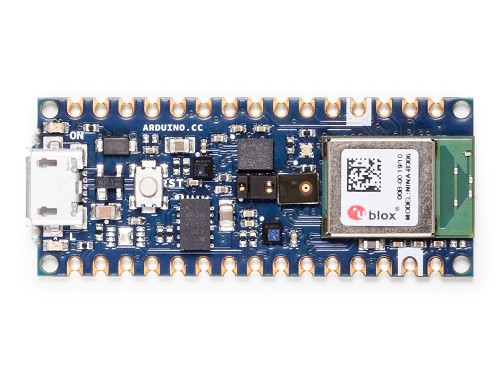
\includegraphics[width=50mm]{Images/Arduino/ArduinoNano33BLESense}
%	
%	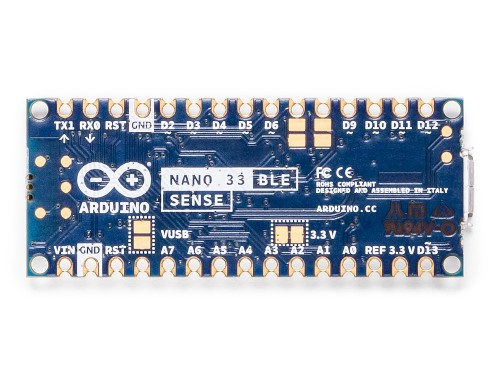
\includegraphics[width=50mm]{Images/Arduino/ArduinoNano33BLESense2}
%	
%	\caption{Arduino Nano 33 BLE Sense \href{https://store.arduino.cc/arduino-nano-33-ble-sense}{Arduino Store}}
%\end{figure}
%
%
%
%
%
%\section{Indroduction}
%
%Arduino has a wide range of Integrated circuit family, depending upon the requirenment and usage. The most commonly available arduino family boards are MKR Family, Arduino Classis, Nano fmaily, Pro Family, and Nicla Family. Each arduino family have further multiple types of boards, e.g the Nano family has a following boards; Nano Classic, Nano 33 BLE, Nano 33 BLE Sense, Nano 33 IoT, and Nano Every, each has a unique specification. The Arduino development board is based on a microcontroller with a large number of standard electronic components and an open source schematic that can be modified as needed.
%
%The BLE (Bluetooth Low Energy) compact and reliable Nano board are built on NINA B306 module for BLE and Bluetooth 5 communication; the NINA B306 module based on Nordic nRF52480 processor that contains a powerful Cortex M4F CPU, Its architecture fully compatible with Arduino IDE Online and Offline. The figure ~\ref{fig:abx00031front12} shows, the Arduino Nano BLE 33 Sense have a following set of sensors on board, ADPS-9960, LPS22HB, HTS221, LSM9DS1,and MP34DT05-A. It is small in size, having all the required sensor on board. \cite{ArduinoNano33:2021}
%
%
%
%\begin{figure}[ht]
%	\centering
%	%\includegraphics[width=0.5\linewidth]{Images/Nano33BLESense/abx00031_front_1_2}
%	\includegraphics[width=0.5\linewidth]{Images/Arduino/abx00031_front_1_2}
%	\caption{Arduino Nano 33 BLE}
%	\label{fig:abx00031front12}
%\end{figure}
%
%The Arduino Nano 33 BLE Sense have the following set of Sensors, BLE module and its functionality below.
%
%\begin{itemize}
%	\item The Bluetooth is managed by a NINA B306 module.
%	\item The ADPS-9960 is a digital proximity, ambient light, RGB and gesture sensor.
%	\item The LSM9DS1 is a system-in-package featuring a 3D digital linear acceleration sensor, a 3D digital angular rate sensor, and a 3D digital magnetic sensor.
%	\item The LPS22HB reads barometric pressure and environmental temperature.
%	\item The HTS221 senses relative humidity.
%	\item The MP34DT05 is support the sound detection.
%\end{itemize}
%
%\section{On Board Sensors and its Functionality}
%
%\subsection{ADPS-9960 (Gesture, Proximity, and Color Detection Sensor)}
%
%The APDS-9960 device features advanced Gesture detection, Proximity detection, Digital Ambient Light Sense (ALS) and Color Sense (RGB). \cite{ArduinoNano33:2021} Gesture detection utilizes four directional photodiodes to sense reflected IR energy (sourced by the integrated LED) to convert physical motion information (i.e. velocity, direction and distance) to a digital information.
%
%
%
%\textbf{Applications}
%
%\begin{itemize}
%	\item Gesture Detection
%	\item Color Sense
%	\item Ambient Light Sensing
%	\item Proximity Sensing
%\end{itemize}
%
%\subsection{LSM9DS1 (Accelerometer, Gyroscope, and Magnetometre)}
%The LSM9DS1 is a system-in-package featuring a 3D digital linear acceleration sensor, a 3D digital angular rate sensor, and a 3D digital magnetic sensor.
%
%\textbf{Aplications}
%
%\begin{itemize}
%	\item Indoor navigation
%	\item Advanced gesture recognition
%	\item Gaming and virtual reality input devices
%	\item Display/map orientation and browsing
%\end{itemize}
%this study will focus mostly on the LSM9DS1 also called IMU see chapter 4 for more details. 
%\subsection{LPS22HB (Pressure Sensor)}
%The LPS22HB is an ultra-compact piezoresistive absolute pressure sensor which functions as a
%digital output barometer.
%
%\textbf{Applications}
%
%
%\begin{itemize}
%	\item Altimeters and barometers for portable devices 
%	\item Weather station equipment
%	\item Sports watchs
%\end{itemize}
%
%\subsection{HTS221 (Relative Humidity and Temperature)}
%The HTS221 is an ultra-compact sensor for relative humidity and temperature. It includes a sensing element and a mixed signal to provide the measurement information through digital serial interfaces.
%
%\textbf{Applications}
%
%\begin{itemize}
%	\item Air conditioning, heating and ventilation 
%	\item Air humidifiers
%	\item Refrigerators
%	\item Smart home automation
%	\item Industrial automation
%\end{itemize}  
%
%
%\subsection{MP34DT05-A (Digital Microphone)}
%
%The MP34DT05-A is an ultra-compact, low-power, omni directional, digital microphone built with a capacitive sensing element and an IC interface. The sensing element, capable of detecting acoustic waves, is manufactured using a specialized silicon micromachining process dedicated to producing audio sensors.
%
%\textbf{Applications}
%
%\begin{itemize}
%	\item Speech recognition 
%	\item Portable media player
%	\item Mobile Terminal
%\end{itemize}
%
%
%\subsection{nRF52840 (Bluetooth Module)}
%
%The nRF52840 is an advanced, highly flexible single chip solution for today’s increasingly demanding Ultra low power (ULP) wireless applications for connected devices on our person, connected living environments and the IoT at large. It is designed ready for the major feature
%advancements of Bluetooth 5 and takes advantage of Bluetooth 5’s increased performance capabilities. \cite{Arduino:2021b}
%
%\textbf{Applications}
%
%\begin{itemize}
%	\item Smart Home products
%	\item Industrial mesh networks
%	\item Smart city infrastructure
%	\item Connected watches
%	\item Advanced personal fitness devices
%	\item Wearables with wireless payment
%	\item Connected Health
%\end{itemize}
%
%The Arduino 33 BLE Sense has a wide range of application, by having the set of sensors and Bluetooth low energy (BLE) capability, the communication becomes easy over the Bluetooth. Arduino Nano 33 BLE Sense operate on 3.3 V, so it make sure that do not apply 5v as normally the other boards need to operate. Also, for making the RGB color and person detection, we need to make the interface of Ble 33 Sense with Arducam OV2640 (Camera Shield). The Arducam OV2640 camera use  to detect the RGB, object detetion and also the gesture too. Arduino Nano 33 BLE Sense and Arducam (camera shield) is a perfect mactch for making ML and AI application, by having the set of sensors on board we just need to install the respective library on Arduino boar and it support the funcnality of sensors and Machine learning application.
%
%\section{Arduino Nano 33 BLE Pin Configuration}
%
%Arduino Nano 33 BLE is an advanced version of Arduino Nano board that is based on a powerful processor the nRF52840. The figure ~\ref{Schnittstellen} shows that the board has the following pin configuration. \href{https://www.etechnophiles.com/arduino-nano-33-ble-sense-pinout-introduction-specifications/}{Pin Configuration}
%
%\textbf{Digital pin:}
%
%The number of digital I/O pins are 14 which receive only two values HIGH or LOW. These pins can either be used as an input or output based on the requirement. When these pins receive 5V, they are in a HIGH state and when they receive 0V they are in a LOW state.
%
%\textbf{Analog pin}
%
%Total 8 analog pins available on the board A0 – A7. These pins get any value as opposed to digital pins that only receive two values HIGH or LOW. These pins are used to measure the analog voltage ranging between 0 to 5V.
%
%
%\textbf{PWM pin}
%
%All digital pins can be used as PWM pins. These pins generate analog results with digital means.
%
%
%\textbf{SPI pin}
%
%The board supports serial peripheral interface (SPI) communication protocol. This protocol is employed to develop communication between a controller and other peripheral devices like shift registers and sensors. Two pins are used for SPI communication i.e. Master Input Slave Output (MISO) and Master Output Slave Input (MOSI) are used for SPI communication. These pins are used to send or receive data by the controller.
%
%\textbf{I2C pin}
%
%The board carries the I2C communication protocol which is a two-wire protocol. It comes with two pins SDL and SCL.
%
%\textbf{UART pin}
%
%The board features a UART communication protocol that is used for serial communication and carries two pins Rx and Tx. The Rx is a receiving pin used to receive the serial data while Tx is a transmission pin used to transmit the serial data.
%
%
%\textbf{External Interrupts pin}
%
%All digital pins can be used as external interrupts. This feature is used in case of emergency to interrupt the main running program with the inclusion of important instructions at that point.
%
%\textbf{LED at Pin 13 and AREF pin}
%
%There is an LED connected to pin 13 of the board. And AREF is a pin used as a reference voltage for the input voltage.
%
%
%
%\begin{figure}[ht]
%	\centering
%	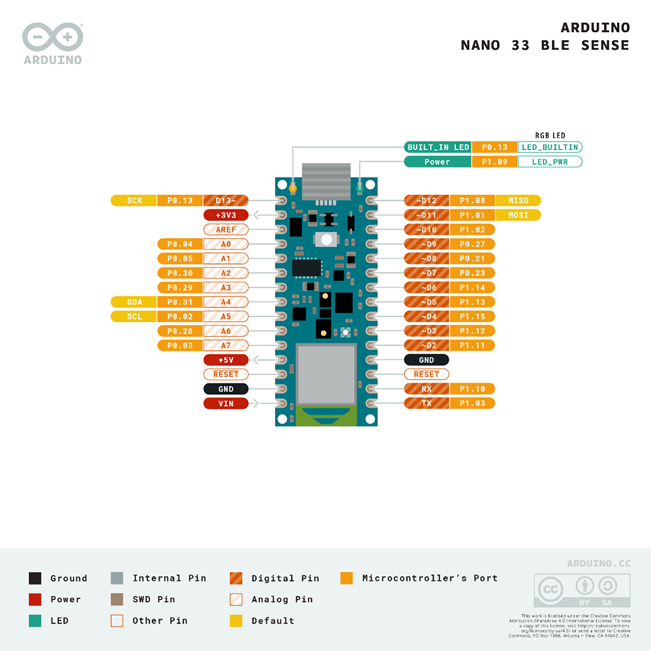
\includegraphics[width=0.5\linewidth]{Images/Arduino/Schnittstellen}
%	\caption{Arduino Nano 33 BLE Pin Configuration}
%	\label{Schnittstellen}
%\end{figure}

\section{Goals of the research}

The primary objective of this research is to develop a cost-effective and accessible solution for tracking gait patterns and identifying disorders. The project, being too complex for a bachelor's thesis, will be divided into two parts. The current phase focuses on monitoring movements of an individual using an Arduino Nano 33 BLE Sense equipped with an IMU sensor placed on the thigh and analyzing the movement in real-time using only the thigh angle and the velocity of the idividual. 

The tool is designed to detect three movements: walking, jumping, and running. Through the use of machine learning, the tool will be able to identify the movement in progress and communicate the result using four labeled LEDs, one for each movement and one for errors (no movement). The final outcome of this research will include:

\begin{itemize}
	\item komplettes gerät: wie soll es aussehen, (HW + SW)
	%\item An introduction to the domain knowledge, including both biological and technical aspects.
	\item A documented workflow: outlining the steps used to find a dataset, select and prepare the data, choose the algorithm, train the model, and upload an optimized version to the board. The documentation aims to make the replication and expansion of the process possible.
	%\item A user guide detailing the function and usage of the tool.
\end{itemize}

The use of an Arduino Nano 33 BLE Sense allows for real-time monitoring and analysis, making it a valuable tool for both research and clinical settings. Ultimately, the goal is to develop a reliable and user-friendly tool that can aid in the early detection and treatment of gait disorders.

\section{Constraints}
%TinyML zitieren
%- Beschränkungen identifizieren : Speicher, Gehäuse, Komplexität, Geschwindigkeit.   
Some constraints must be considered such as the limited memory available and the power of the device, the memory on microcontrollers are usually limited as well as their power, this include the used Arduino Nani 33 BLE Board. thus it is not possible to train the model on the board and only a compressed version of the model will be uploaded into our board. the creation initialisation and training will accure on a computer. 
\cite{ArduinoNano33BLESense:2023}

Another thing to pay attention to is the Energy source, the end device is supposed to be wearable, Arduino boards are usually powered through an USB Port but can also be powered through..., 
two possible ways are open to us, either use a Powerbank and connect it to the device, which will allow the user to recharge the Tool when needed, or we can use a simple 9V battery that will need to be changed when empty. 
Employing a battery eliminates the uncertainty of device detection by a power bank, particularly in low energy consumption scenarios. While it is possible to modify the power bank's device detection feature, this approach would entail additional time and resources.\\
The design and construction of the device housing must be evaluated to ensure the integrity of the internal components, particularly in the event of a fall or exposure to outdoor conditions such as rain. Additionally, the housing should include provision for LED lights, including appropriate labeling to indicate their function, as well as a means of turning the device on and off.\\

Lastly, it is important to acknowledge the complexity of the project and the fact that none of the project participants possess prior experience with microcontrollers, sensors, or the practical application of machine learning, which increases the duration needed for the project.

\section{Structure}

This paper is focused on the development of a system for recognizing human locomotion using an Arduino Nano 33 BLE Sense microcontroller and machine learning algorithms.
you will be able to find the domain knowlage both technical and biological needed in orded to develop the system.


in chapter \ref{Introduction} .Introduction we get a general explenation of the reasons of the research its goals and the constraints that comes with it. 

As we dive into the next chapter \ref{Human gait pattern} , labeled as "Human Gait Pattern," we come across valuable knowledge pertaining to the physiology of the human body. This knowledge proves to be essential for the project at hand. The chapter starts off by providing us with a general explanation of the human gait pattern, which includes a detailed breakdown of the various phases of a gait cycle, as documented in Perry's study in 1992 \ref{Perry:1992}.

Moving forward, the second part of the chapter focuses on the distinct characteristics of different human locomotions, such as walking, running, standing, and sitting. The goal is to showcase the differences between these modes of locomotion and to highlight the links between these variations and an IMU measurement system.  
 
In the  \ref{Hardware} chapter of the project, we delve into the hardware used for this project. The main board used for the project is the Arduino Nano 33 BLE Sense. This section provides valuable insights into the integrated sensors available on the board, which includes the IMU sensor.
 
Additionally, this chapter covers the pin configuration of the board and offers details on how an IMU measurement system can be calibrated. 

Moreover, this chapter also sheds light on the different power sources compatible with the device. Understanding the power source compatibility is essential as it helps to determine the device's battery life and overall power consumption.
 
Overall, this chapter serves as an essential guide to the hardware used in the project, offering a comprehensive overview of the various components used, their configuration, and the possible power sources.
 
 
In the fifth section \ref{Software} of the project, we shift our focus towards the software aspect. This section covers the various software tools required for the project, including the Arduino IDE on PC, Python installation, and the Anaconda supporting framework for Jupyter Notebook.
 
The chapter starts by detailing the installation process of the Arduino IDE on PC. This software is essential for programming the Arduino Nano 33 BLE Sense board, and this section guides us through the necessary steps required to install and configure the software for our project as well as the upload of the program on the board.
 
The next part of the chapter discusses the Python installation required for the project. Python is a widely used programming language that can be used for data analysis and visualisation. 
This section provides an overview of the installation process, highlighting the key aspects that are relevant to our project.
 
Finally, the chapter concludes with details on the Anaconda supporting framework for Jupyter Notebook. This software framework provides a platform for interactive data analysis and visualization. The section highlights the importance of this framework for our project and guides us through the installation process.
 Overall, this section provides a comprehensive overview of the various software tools required for the project, offering step-by-step guidance on their installation and configuration.

The  \ref{TFandTML} chapter of the project is focused on introducing machine learning and its application in our project. The chapter starts with an overview of TensorFlow, a widely used open-source machine learning framework. The section provides a brief overview of the framework and its functionalities.

it delves into TinyML, a specialized version of machine learning designed for low-power devices such as the Arduino Nano 33 BLE Sense. The section provides an overview of the TinyML workflow and how it can be used to develop machine learning models for our project.
The chapter then introduces three algorithms that are compatible with our project and provides guidance on how to select the best algorithm for our needs. we get also a theoretical explanation of how to train a machine learning model, an explantion of  how to convert the machine learning model with TensorFlow Lite, a lightweight version of TensorFlow designed for mobile and embedded devices and a guidance on how to export the machine learning model and load it onto the Arduino Nano 33 BLE Sense board with TensorFlow micro.

In the \ref{Datasets} chapter of the project, we explore the different datasets that are suitable for our project. This section provides detailed information on the Wireless Sensor Data Mining (WISDM) dataset, the UCI Human Activity Recognition dataset, and the OPPORTUNITY++ dataset.

Each dataset is examined in terms of its advantages and limitations, and its suitability for our project is assessed. The section explains that the WISDM dataset is compatible with our project requirements and is suitable for developing a machine learning model for gesture recognition on the Arduino Nano 33 BLE Sense board. 

The chapter labeled as \ref{KDD} presents a comprehensive description of the knowledge discovery in databases (KDD) methodology, also known as the KDD process. Meanwhile, the final chapter, \ref{KDDP}, offers a detailed, step-by-step guide on how to implement the KDD process in our project. This covers both the development component, including data collection and evaluation, and the deployment aspect, which involves testing the hardware, implementing the machine learning pipeline, deploying the application, and monitoring the system. Essentially, this chapter provides a practical approach to implementing the KDD process in real-world scenarios.



